% -*- root: main.tex -*-

\chapter{The $\sigma$-orientation}\label{ChapterSigmaOrientation}


\todo[inline]{Write an introduction for me.  Use unstable cooperations from Morava's theories to classical complex and real $K$--theory.}

\todo[inline]{Part of the theme of this chapter should be to use the homomorphism from topological vector bundles to algebraic line bundles --- Neil's $\mathbb L$ construction --- as inspiration for what to do, given suitable algebraic background.}

\todo[inline]{An artifact of these being lecture notes for an actual class is that this last section is getting compressed due to end-of-semester time constraints.  I think a published version of these notes would contain proofs of a bunch of these facts which, at present, are getting omitted either because the proofs take too long or because simply understanding the theorem statements takes too long.  Really, the class in general is becoming quite strained at this point: it's hard to keep everything straight both for the students and for the teacher.}




\section{Coalgebraic formal schemes}

Today we will discuss an elephant that has been lingering in our room: we began the class talking about the formal scheme associated to the \emph{cohomology} of a space, but we have since become primarily interested in a construction converting the \emph{homology} of a spectrum to a sheaf over a context.  Our goal for today is to, when possible, put these on even footing.  Our motivation for finally addressing this lingering discrepancy is more technical than aesthetic: we have previously wanted access to certain colimits of formal schemes (e.g., in \Cref{DivConstructionsAreFree}).  While such colimits are generally forbidding, similarly to colimits of manifolds, we will produce certain conditions under which they are accessible.

Suppose that $E$ is a ring spectrum, and recall the usual way to produce the structure of an $E^*$--algebra on $E^* X$ for $X$ a space.  The space $X$ has a diagonal map $\Delta\co X \to X \times X$, which on $E$--cohomology induces a multiplication map \[E^* X \otimes_{E^*} E^* X \xrightarrow{\mu_E} E^*(X \times X) \xrightarrow{E^* \Delta} E^* X.\]  Dually, applying $E$--homology, we have a pair of maps \[E_* X \xrightarrow{E_* \Delta} E_*(X \times X) \xleftarrow{\text{K\"unneth}} E_* X \otimes_{E_*} E_* X.\]  In the case that the K\"unneth map is an isomorphism, the right--hand map is invertible, and the long composite induces the structure of an $E_*$--coalgebra on $E_* X$.  In the most generous case that $E$ is a field spectrum (in the sense of \Cref{FieldSpectraAreKTheories}), $E^* X$ is functorially the linear dual of $E_* X$, which motivates us to consider the following purely algebraic construction:

\begin{definition}
Let $C$ be a coalgebra over a field $k$.  The scheme $\Sch C$ associated to $C$ is defined by \[(\Sch C)(T) = \left\{f \in C \otimes T \middle| \begin{array}{c} \Delta f = f \otimes f \in (C \otimes T) \otimes_T (C \otimes T), \\ \eps f = 1 \end{array} \right\}.\]
\end{definition}

\begin{lemma}
For $A$ a $k$--algebra, finite--dimensional as a $k$--module, one has $\Spec A \cong \Sch A^*$.
\end{lemma}
\begin{proof}[Proof sketch]
A point $f \in (\Sch A^*)(T) \subseteq A^* \otimes T$ gives rise to a map $f_*\co A \to T$ by the duality pairing, which is a ring homomorphism by the condition.  The finiteness assumption is present exactly so that $A$ is its own double--dual, giving an inverse assignment.
\end{proof}

If we drop the finiteness assumption, then a lot can go wrong.  For instance, the multiplication on our $k$--algebra $A$ gives rise only to maps \[A^* \to (A \otimes_k A)^* \from A^* \otimes_k A^*,\] which is not enough to make $A^*$ into a $k$--coalgebra.  However, if we start instead with a $k$--coalgebra $C$ of infinite dimension, the following result is very telling:

\begin{lemma}\label{kCoalgebrasAreIndFinite}\citeme{Demazure's book has this somewhere in it, also see your thesis for a more modern reference}
For $C$ a coalgebra over a field $k$, any finite--dimensional $k$--linear subspace of $C$ can be finitely enlarged to a subcoalgebra of $C$.  Accordingly, taking the colimit gives a canonical equivalence \[\Ind(\CatOf{Coalgebras}_k^{\mathrm{fin}}) \xrightarrow{\simeq} \CatOf{Coalgebras}_k. \qed\]
\end{lemma}

\noindent This result allows us to leverage our duality Lemma pointwise: for an arbitrary $k$--coalgebra, we break it up into a lattice of finite $k$--coalgebras, and take their linear duals to get a reversed lattice of finite $k$--algebras.  Altogether, this indicates that $k$--coalgebras generally want to model \emph{formal schemes}.

\begin{corollary}\label{CoalgsAndFSchsAgreeOverk}
For $C$ a coalgebra over a field $k$ expressed as a colimit $C = \colim_k C_k$ of finite subcoalgebras, there is an equivalence \[\Sch C \cong \{\Spec C_k^*\}_k.\]  This induces a \emph{covariant} equivalence of categories \[\CatOf{Coalgebras}_k \cong \CatOf{FormalSchemes}_{/k}. \qed\]
\end{corollary}

This covariant algebraic model for formal schemes is very useful.  \todo{Do you also need to compare the (Cartesian) monoidal structures?}  For instance, this equivalence makes the following calculation trivial:
\begin{lemma}[{(cf.\ \Cref{DivConstructionsAreFree} and )}]\todo{Backreference the relevance of the $\Div$ construction to homotopy theory.}
Select a coalgebra $C$ over a field $k$ together with a pointing $k \to C$.  Write $M$ for the coideal $M = C / k$.  The free formal monoid on the pointed formal scheme $\Sch k \to \Sch C$ is given by \todo{Describe the diagonal map on this guy.} \[F(\Sch k \to \Sch C) = \Sch \Sym^* M. \qed\]
\end{lemma}

It is unfortunate, then, that when working over an object more general than a field \Cref{kCoalgebrasAreIndFinite} fails.\todo{Include (a reference to) an example.}  Nonetheless, it is possible to bake into the definitions the machinery needed to get a good-enough analogue of \Cref{CoalgsAndFSchsAgreeOverk}.

\begin{definition}
Let $C$ be an $R$--coalgebra which is free as an $R$--module.  A basis $\{x_j\}$ of $C$ is said to be a \textit{good basis} when any finite subcollection of $\{x_j\}$ can be finitely enlarged to a subcollection that spans a subcoalgebra.  The coalgebra $C$ is itself said to be \textit{good} when it admits a good basis.  A formal scheme $X$ is said to be \textit{coalgebraic} when it is isomorphic to $\Sch C$ for a good coalgebra $C$.
\end{definition}

\begin{theorem}[{\cite[Proposition 4.64]{StricklandFSFG}}]\label{CoalgebraicColimitsExist}
Suppose that $F\co \CatOf I \to \CatOf{Coalgebras}_R$ is a colimit diagram of coalgebras such that each object in the diagram, including the colimit point, is a good coalgebra.  Then \[\Sch \circ F\co \CatOf I \to \CatOf{FormalSchemes}\] is a colimit diagram of formal schemes. \qed
\end{theorem}

This Theorem gives us access to many constructions on formal schemes, provided we assume that the input is coalgebraic.  This covers many of the cases of interest to us, as every formal variety is coalgebraic.  For an example of the sort of constructions that become available, one can prove the following Corollary by analyzing the symmetric power of coalgebras:

\begin{corollary}[{\cite[Proposition 6.4]{StricklandFSFG}}]
For $X$ a coalgebraic formal scheme, $X^{\times n}_{\Sigma_n}$ exists.  In fact, $\coprod_{n \ge 0} X^{\times n}_{\Sigma n}$ models the free formal monoid on $X$.  If $\Spec k \to X$ is a pointing, then $\colim_n \{X^{\times n}_{\Sigma_n}\}_n$ models the free formal monoid on the pointed formal scheme. \qed
\end{corollary}

In the specific case that $\Spec k \to X$ is a formal \emph{curve}, we can prove something more:
\begin{corollary}[{\cite[Proposition 6.13]{StricklandFSFG}}]
For $\Spec k \to X$ a pointed formal curve, the free formal monoid is automatically an abelian group. \qed
\end{corollary}
\begin{proof}[Proof sketch]
The idea is that the symmetric algebra on the coalgebra associated to a formal curve admits a sufficiently nice filtration that one can iteratively solve for a Hopf algebra antipode.
\end{proof}

We now reconnect this algebraic discussion with the algebraic topology that spurred it.

\begin{lemma}
If $E$ and $X$ are such that $E_* X$ is an $E_*$--coalgebra and \[E^* X = \CatOf{Modules}_{E_*}(E_* X, E_*),\] then there is an equivalence \[\Sch E_* X \cong X_E. \qed\]
\end{lemma}
\begin{proof}[Proof sketch]
The main point is that the formal topology on $X_E$ is induced by the compactly generated topology of $X$, and this same topology can also be used to write $\Sch E_* X$ as the colimit of finite $E_*$--coalgebras.
\end{proof}

\begin{example}[{\Cref{KtheoryConvertsTorsionToTorsion} and \Cref{KHomologyOfClassifyingSpace}}]
For a Morava $K$--theory $K_\Gamma$ associated to a formal group $\Gamma$ of finite height, we have seen that there is an exact sequence of Hopf algebras \[K_\Gamma^0(BS^1) \xrightarrow{[p^j]} K_\Gamma^0(BS^1) \to K_\Gamma^0(BS^1[p^j]),\] presenting $(BS^1[p^j])_K$ as the $p^j$--torsion formal subscheme $BS^1_K[p^j]$.  The Hopf algebra calculation also holds in $K$--homology, where there is instead the following exact sequence \[(K_\Gamma)_0 B(S^1[p^j]) \to (K_\Gamma)_0 BS^1 \xrightarrow{(-)^{\ast p^j}} (K_\Gamma)_0 BS^1,\] presenting $(K_\Gamma)_0 B(S^1[p^j])$ as the $p^j$--order $\ast$--nilpotence in the middle Hopf algebra.  Applying $\Sch$ to this last line covariantly converts this second statement about Hopf algebras to the corresponding statement above about the associated formal schemes --- i.e., the behavior of the homology coalgebra is a direct reflection of the behavior of the formal schemes.
\end{example}

The example above also spurs us to consider an intermediate operation.  We have seen that the algebra structure of the $K$--cohomology of a space and the coalgebra structure of the $K$--homology of the same space contain equivalent data: they both give rise to the same formal scheme.  However, in the case at hand, $BS^1$ and $BS^1[p^j]$ are commutative $H$--spaces and hence give rise to \emph{commutative and cocommutative Hopf algebras} on both $K$--cohomology and $K$--homology.  Hence, in addition to considering the coalgebraic formal scheme $\Sch (K_\Gamma)_0 B(S^1[p^j])$, we can also consider the affine scheme $\Spec (K_\Gamma)_0 B(S^1[p^j])$.  This, too, should contain identical information, and this is the subject of Cartier duality.

\begin{definition}[{\cite[Section 6.4]{StricklandFSFG}}]
The \textit{Cartier dual} of a finite group scheme $G$ is defined by \[DG = \InternalHom{GroupSchemes}(G, \Gm).\]
\end{definition}

\begin{lemma}[{\cite[Proposition 6.19]{StricklandFSFG}}]
On the level of Hopf algebras $A = \sheaf O_G$, this has the effect \[DG = \Sch A = \Spec A^*. \qed\]
\end{lemma}
\todo{You could stand to include a proof of this.  It's been a while since you actually proved something serious with formal schemes, and this is pretty nice.}

\todo{You could also include mention of the motivation: $C_k \G$ is hard to exhibit, but $(C_k \G)^\vee$ is easy.  It's not clear how to do this without leaping too far ahead, though.}

\begin{remark}
The effect of Cartier duality on the Dieudonn\'e module of a formal group is linear duality.  Hence, the covariant and contravariant Dieudonn\'e modules described in \Cref{SectionDieudonneModules} are related by Cartier duality.
\end{remark}

\begin{remark}\label{TopologicalCartierDuality}
The topological summary of Cartier duality is that, when $X$ is a free even commutative $H$--space, \[DX_E = \InternalHom{GroupSchemes}(X_E, \Gm) = \Spec E_0 X.\]
\end{remark}












\section{Special divisors and the special splitting principle}\label{MSUDay}

\todo{You should be a little careful here: are the Triumvirate theorems a little stronger than the culmination of (1), (2), and (3)? I think the proof of the equivalence of (2) and (3) on $T$--points rather than on $E_0$--points is something slightly harder than the most basic equivalence between (2) and (3) (which concerns only $E_0$--points).}

Starting today, after our extended interludes on chromatic homotopy theory and cooperations, we are going to return to thinking about bordism orientations directly.  To begin, we will recall the various perspectives adopted in \Cref{ComplexBordismChapter} when we were studying complex--orientations of ring spectra.
\begin{enumerate}
\item A complex--orientation of $E$ is, definitionally, a map $MUP \to E$ of ring spectra in the homotopy category.
\item A complex--orientation of $E$ is also equivalent to a multiplicative system of Thom isomorphisms for complex vector bundles.  Such a system is determined by its value on the universal line bundle $\L$ over $\CP^\infty$.  We can also phrase this algebro-geometrically: such a Thom isomorphism is the data of a trivialization of the Thom sheaf $\ThomSheaf{\L}$ over $\CP^\infty_E$.
\item Ring spectrum maps $MUP \to E$ induce on $E$--homology maps $E_0 MUP \to E_0$ of $E_0$--algebras.  This, too, can be phrased algebro-geometrically: these are elements of $(\Spec E_0 MUP)(E_0)$.
\end{enumerate}
We can summarize our main result about these perspectives as follows:
\begin{theorem}[{\cite[Example 2.53]{AHSTheoremOfTheCube}}]\label{BUZTriumvirate}\citeme{Put in cross references}
Take $E$ to be \emph{complex--orientable}.  The functor
\begin{align*}
\CatOf{AffineSchemes}_{/\Spec E_0} & \to \CatOf{Sets}, \\
(\Spec T \xrightarrow{u} \Spec E_0) & \mapsto \left\{ \text{trivializations of $u^* \ThomSheaf{\L}$ over $u^* \CP^\infty_E$} \right\}
\end{align*}
is isomorphic to the affine scheme $\Spec E_0 MUP$.  Moreover, the $E_0$--points of this scheme biject with ring spectrum maps $MUP \to E$.
\end{theorem}
\begin{proof}[Proof summary]
The equivalence between (1) and (2) is given by the splitting principle for complex line bundles.  The equivalence between (1) and (3) follows from calculating that $E_0 MUP$ is a free $E_0$--module.
\end{proof}

An analogous result holds for ring spectrum maps $MU \to E$ and the line bundle $\L - 1$, and it is proven in analogous way.  In particular, we will want a version of the splitting principle for virtual vector bundles of virtual rank $0$.  Given a finite complex $X$ and such a rank $0$ virtual vector bundle, write \[\tilde V \co X \to BU\] for the classifying map.  Because $X$ is a finite complex, there exists an integer $n$ so that $\tilde V = V - n \cdot 1$ for an honest rank $n$ vector bundle $V$ over $X$.  Using \Cref{OriginalSplittingPrinciple}, the splitting $f^* V \cong \bigoplus_{i=1}^n \L_i$ over $Y$ gives a of $\tilde V$ \emph{internally to $BU$} as \[\tilde V = V - n \cdot 1 = \bigoplus_{i=1}^n (\L_i - 1),\] as each bundle $\L_i - 1$ itself has the natural structure of a rank $0$ virtual vector bundle.  This begets the following analogue of the previous result:
\begin{theorem}[{\cite[Example 2.54]{AHSTheoremOfTheCube}}]\label{BUTriumvirate}\citeme{Put in cross references}
Take $E$ to be complex--orientable.  The functor
\begin{align*}
\CatOf{AffineSchemes}_{/\Spec E_0} & \to \CatOf{Sets}, \\
(\Spec T \xrightarrow{u} \Spec E_0) & \mapsto \left\{ \text{trivializations of $u^* \ThomSheaf{\L - 1}$ over $u^* \CP^\infty_E$} \right\}
\end{align*}
is isomorphic to the affine scheme $\Spec E_0 MU$.  Moreover, the $E_0$--points of this scheme biject with ring spectrum maps $MU \to E$. \qed
\todo{Identify this bundle $\ThomSheaf{\L - 1}$ as $\omega \otimes \sheaf I(0)^{-1}$, we can think of sections as elements of $E^0 T(\L - 1 \to \CP^\infty)$ which restrict to the identity under the inclusion \[S^0 \to P^{\L-1}.\]}
\end{theorem}

\begin{remark}
The map $BU \to BU \times \Z$ induces a map $MU \to MUP$.  The induced map on schemes is normalization:\todo{Justify this.}
\begin{align*}
\Spec E_0 MUP & \to \Spec E_0 MU, \\
f & \mapsto \frac{f'(0)}{f}.
\end{align*}
\end{remark}

These two Thom spectra are the beginning of a larger pattern.  Their base spaces $BU \times \Z$ and $BU$ are both infinite loopspaces: they are $\OS{kU}{0}$ and $\OS{kU}{2}$ respectively, where $kU$ is the connective complex $K$--theory spectrum.  In general, the space $\OS{kU}{2k}$ is given as a connective cover\todo{Justify this as a Lemma.}: \[\OS{kU}{2k} = BU[2k, \infty),\] and so the next Thom spectrum in the sequence is $MSU$, the bordism theory of $SU$--structured manifolds.  The special unitary group $SU$ is explicit enough that these orientations can be fully understood along similar lines to what we have done so far.  Our jumping off point for that story will be, again, an extension of the splitting principle.
\begin{lemma}\label{SplittingPrincipleForBSU}
\todo{Hood had a question here: what symmetry group acts on this splitting? I think it's possible to show that the full symmetric group action on the $BU \times \Z$ splitting induces a full symmetric group action on the $BSU$ splitting. I don't know if there's any more or any less.}
Let $X$ be a finite complex, and let $\tilde V\co X \to BU$ classify a virtual vector bundle of rank $0$ over $X$.  Select a factorization $\tilde{\tilde V}\co X \to BSU$ of $\tilde V$ through $BSU$.  Then, there is a space $f\co Y \to X$, where $f_E\co Y_E \to X_E$ is finite and flat, as well as a collection of line bundles $\sheaf H_j$, $\sheaf H'_j$ expressing a $BSU$--internal decomposition \[\tilde{\tilde V} = -\bigoplus_{j=1}^n (\sheaf H_j - 1)(\sheaf H'_j - 1).\]
\end{lemma}
\begin{proof}
Begin by using \Cref{OriginalSplittingPrinciple} on $V$ to get an equality of $BU$--bundles \[\tilde{\tilde V} = V' + \L_1 + \L_2 - n \cdot 1.\]  Adding $(\L_1 - 1)(\L_2 - 1)$ to both sides, this gives
\begin{align*}
\tilde{\tilde V} + (\L_1 - 1)(\L_2 - 1) & = V' + \L_1 + \L_2 + (\L_1 - 1)(\L_2 - 1) - n \cdot 1 \\
& = V' + \L_1\L_2 - (n-1) \cdot 1.
\end{align*}
By thinking of $(\L_j - 1)$ as an element of $kU^2(Y) = \CatOf{Spaces}(Y, BU)$, we see that the product element $(\L_1 - 1)(\L_2 - 1) \in kU^4(Y) = \CatOf{Spaces}(Y, BSU)$ has the natural structure of a $BSU$--bundle and hence so does the sum on the left-hand side\footnote{In the language of last section, we are making use of the Hopf ring $\circ$--product.}.  The right-hand side is the rank $0$ virtualization of a rank $(n-1)$ vector bundle, hence succumbs to induction.  Finally, because $SU(1)$ is the trivial group, there are no nontrivial complex line bundles with structure group $SU(1)$, grounding the induction.
\end{proof}

\begin{corollary}
Ring spectrum maps $MSU \to E$ biject with trivializations of \[\ThomSheaf{(\L_1 - 1)(\L_2 - 1)} \downarrow (\CP^\infty)^{\times 2}_E. \qed \]
\end{corollary}

\begin{remark}\label{TwoCocycleConditionForBSUBundles}
Since we used the product map \[kU^2(Y) \otimes kU^2(Y) \to kU^4(Y)\] in the course of the proof, it is also interesting to consider the product map \[kU^4(Y) \otimes kU^0(Y) \to kU^4(Y).\]  Taking one of our splitting summands $(\L_1 - 1)(\L_2 - 1)$ and acting by some line bundle $\sheaf H$ gives
\begin{align*}
(\L_1-1)\sheaf H(\L_2 - 1) & = \\
(\sheaf H \L_1 - \sheaf H)(\L_2 - 1) & = (\L_1-1)(\sheaf H \L_2 - \sheaf H) \\
(\sheaf H \L_1 - 1)(\L_2 - 1) - (\sheaf H - 1)(\L_2 - 1) & = (\L_1 - 1)(\sheaf H \L_2 - 1) - (\L_1 - 1)(\sheaf H - 1).
\end{align*}
This ``$kU^0$--linearity'' is sometimes called a ``$2$--cocycle condition'', in reference to the similarity with the formula in \Cref{DefinitionSymmetric2Cocycle}.
\end{remark}

If we can show that $E_* BSU$ is even--concentrated and free as an $E_0$--module, then this will complete the $BSU$--analogue of \Cref{BUZTriumvirate,BUTriumvirate}.  This is quite easy, following directly from the Serre spectral sequence:
\begin{lemma}[{\cite[Lemma 6.1]{AndoStrickland}}]\label{BSUtoBUtoCPinftyIsSexseq}
The Postnikov fibration \[BSU \to BU \xrightarrow{B\det} BU(1)\] induces a short exact sequence of Hopf algebras \[E^0 BSU \from E^0 BU \xleftarrow{c_1 \mapsfrom c_1} E^0 BU(1). \qed\]
\end{lemma}
\begin{corollary}\label{BSUTriumvirate}
The functor \[\{\Spec T \xrightarrow{u} \Spec E_0\} \to \left\{ \text{trivializations of $u^* \ThomSheaf{(\L_1 - 1)(\L_2 - 1)}$ over $u^* \CP^\infty_E$} \right\}\] is isomorphic to the affine scheme $\Spec E_0 MSU$.  Moreover, the $E_0$--points of this scheme biject with ring spectrum maps $MSU \to E$. \qed
\end{corollary}

However, the use of \Cref{BSUtoBUtoCPinftyIsSexseq} inspires us to spend a moment longer with the associated formal schemes.  An equivalent statement is that there is a short exact sequence of formal group schemes
\begin{center}
\begin{tikzcd}
BSU_E \arrow{r} \arrow[equal]{d} & BU_E \arrow{r}{B\det} \arrow[equal]{d} & BU(1) \arrow[equal]{d} \\
\SDiv_0 \CP^\infty_E \arrow{r} & \Div_0 \CP^\infty_E \arrow{r}{\mathrm{sum}} & \CP^\infty_E,
\end{tikzcd}
\end{center}
where the scheme ``$\SDiv_0 \CP^\infty$'' of ``special divisors'' consists of those divisors which vanish under the summation map.  However, where the comparison map $BU(1)_E \to BU_E$ has an identifiable universal property --- it presents $BU_E$ as the universal formal group on the pointed curve $BU(1)_E$ --- the description of $BSU_E$ as a scheme of special divisors does not bear much immediate resemblance to a free object on the special divisor $([a] - [0])([b] - [0])$ classified by \[(\CP^\infty)^{\times 2}_E \xrightarrow{(\L_1 - 1)(\L_2 - 1)_E} BSU_E \to BU_E = \Div_0 \CP^\infty_E.\]  It would be wise of us to straighten this out before moving on.

\begin{definition}\label{DefinitionOfC2G}
If it exists, let $C_2 \G$ denote the symmetric square of $\Div_0 \G$, thought of as a module over $\Div \G$.  This scheme has the property that a formal group homomorphism $\phi\co C_2 \G \to H$ is equivalent data to a symmetric function $\psi\co \G \times \G \to H$ satisfying a rigidity condition ($\psi(x, 0) = 0$)\todo{Allen wanted to know why this deserved to be called ``rigid''.} and a $2$--cocycle condition as in \Cref{TwoCocycleConditionForBSUBundles}.
\end{definition}

\begin{theorem}[{Ando--Hopkins--Strickland, unpublished}]\label{SDivModelsC2}\citeme{This is Prop 3.2 of the AHS preprint or Prop 2.13 of Strickland's FSKS preprint}
$\SDiv_0 \G$ is a model for $C_2 \G$.
\end{theorem}
\begin{proof}[Proof sketch]
Consider the map
\begin{align*}
\G \times \G & \to \Div_0 \G, \\
(a, b) & \mapsto ([a] - [0])([b] - [0])
\end{align*}
for which there is a factorization of formal schemes
\begin{center}
\begin{tikzcd}
\G \times \G \arrow[densely dotted]{d} \arrow{rd} \\
F \arrow{r}{\ker} & \Div_0 \G \arrow{r}{\sigma} & \G
\end{tikzcd}
\end{center}
because \[\sigma(([a] - [0])([b] - [0])) = (a + b) - a - b + 0 = 0.\]  One can check that a homomorphism $F \to H$ pulls back to a function $\G \times \G \to H$ satisfying the properties of \Cref{DefinitionOfC2G}.  To go the other way\footnote{To get insight into how this part of the proof works, actually write out the expressions for $\tilde{\tilde{V}} = \bigoplus_{i=1}^6 \L_i - 6 \cdot 1 = \bigoplus_{i=1}^3 (\L_i - 1) \oplus \bigoplus_{j=4}^6 (\L_j - 1)$ and see what happens.}, we select a function $\psi\co \G \times \G \to H$ and mimic the construction in \Cref{SplittingPrincipleForBSU}.  Expanding the definition of $\Div_0 \G$, we are moved to consider the object $\G^{\times k}$ parametrizing weight $k$ divisors with a full set of sections\todo{You can say this better, right? Do you need the thing to have a full set of sections to define this map? Probably not...}, where we define a map
\begin{align*}
\G^{\times k} & \to H, \\
(a_1, \ldots, a_k) & \mapsto -\sum_{j=2}^k \psi\left(\sum_{i=1}^{j-1} a_i, a_j \right).
\end{align*}
This gives a compatible system of symmetric maps and hence bundles together to give a map $\tilde\phi\co\Div_0 \G \to H$ off of the colimit.  In general, this map is not a homomorphism, but it is a homomorphism when restricted to $\phi\co F \to \Div_0 \G \to H$.  Finally, one checks that any homomorphism $F \to H$ of formal groups restricting to the zero map $\G \times \G \to H$ was already the zero map, and this gives the desired identification of $F$ with the universal property of $C_2 \G$.
\end{proof}

In the next interesting case of $\OS{kU}{6} = BU[6, \infty)$, there is not an accessible splitting principle.  This not only makes the topology harder, but it also makes proving the existence of the symmetric cube $C_3 \G$ harder, as there is no model to work from.  Nonetheless, there is a $BU[6, \infty)$--analogue of \Cref{BUZTriumvirate}, \Cref{BUTriumvirate}, and \Cref{BSUTriumvirate}.  In order to prove it, since we don't have access to an equivalence between viewpoints (1) and (2), we will have to instead prove an equivalence between (2) and (3) directly.




\todo{There's some stuff buried here about moving to the Thom spectrum after doing the analysis of the classifying space.  I'm not sure where it lives just yet.}

% Before embarking on this much harder case, we would be wise to investigate how such an equivalence works in the case of $MSU$.


% \citeme{Ando--Hopkins--Strickland 2.4.5}
% There is a map of schemes \[\Spec E_0 MSU \xrightarrow{g_2} C^2(\G; \sheaf I(0))\] which is a map of torsors compatible with the action maps
% \begin{center}
% \begin{tikzcd}
% \Spec E_0 MSU \times_{S_E} \Spec E_0 BSU \arrow{r} \arrow{d} & \Spec E_0 MSU \arrow{d} \\
% C^2(\G_E; \sheaf I(0)) \times C^2(\G_E; \sheaf O) \arrow{r} & C^2(\G_E; \sheaf I(0) \otimes_{\sheaf O} \sheaf O).
% \end{tikzcd}
% \end{center}
% The net effect is that this map $g_2$ is automatically an isomorphism.

% \todo{Write these elements of $C^2$ as sections of the bundle $\Theta^2 \L$.  Note that this construction is monoidal.}

% \begin{remark}
% Even without access to $C_2 \G$, the scheme \[C^2(\G; \sheaf O) = \InternalHom{FormalSchemes}(C_2 \G, \Gm) = (C_2 \G)^\vee\] is directly accessible.  By picking a coordinate on $\G$, points of the middle scheme have presentations of power series satisfying particular identities, hence immediately exist as an affine scheme.
% \end{remark}

% \begin{remark}
% The map $MSU \to MU$ on affine schemes is given by
% \begin{align*}
% \Spec E_0 MU & \to \Spec E_0 MSU, \\
% f(x) & \mapsto \frac{f(x + y)}{f(x) \cdot f(y)}.
% \end{align*}
% \end{remark}


% Identify the Thom sheaf of the universal bundle on $BSU$ as $C^2(\G; \sheaf I(0))$, together with its $C^2(\G, \Gm)$--torsor structure, and note that this automatically promotes the classifying map $MSU^E \to C^2(\G; \sheaf I(0))$ to an isomorphism.










\section{Elliptic curves and $\theta$--functions}\label{SectionEllipticCurvesAndThetaFunctions}

\todo{The goal of this lecture should be to set up all the algebraic geometry we'll need, in a coherent-enough way that the students will be able to think back and at least mumble ``yeah, ok, reasonable''.}

Today will constitute something of a r\'esum\'e on elliptic curves.  We'll hardly prove anything, and we also won't cover many topics that a sane introduction to elliptic curves would make a point to cover.  Instead, we'll try to restrict attention to those concepts which will be of immediate use to us in the coming couple of lectures --- in particular, we will discover a place where ``$C_3 \G$'' appears internally to the theory of elliptic curves.

To begin with, recall that an elliptic curve in the complex setting is a torus, and it admits a presentation by selecting a lattice $\Lambda$ of full rank in $\C$ and forming the quotient \[\C \xrightarrow{\pi_\Lambda} E_\Lambda = \C / \Lambda.\]  The meromorphic functions $f$ on $E_\Lambda$ pull back to give meromorphic functions $\pi_\Lambda^* f$ on $\C$ satisfying a periodicity constraint in the form of the functional equation \[\pi_\Lambda^* f(z + \Lambda) = \pi_\Lambda^* f(z).\]  From this, it follows that there are no holomorphic such functions, save the constants --- such a function would be bounded, and Liouville's theorem would apply.  It is, however, possible to build the following meromorphic special function, which has poles of order $2$ at the lattice points: \[\wp_\Lambda(z) = \frac{1}{z^2} + \sum_{\omega \in \Lambda \setminus \{0\}} \frac{1}{(z - \omega)^2} - \frac{1}{\omega^2}.\]  Its derivative is also a meromorphic function satisfying the periodicity constraint: \[\wp_\Lambda'(z) = -2 \sum_{\omega \in \Lambda} \frac{1}{(z - \omega)^3}.\]  In fact, these two functions generate all other meromorphic functions on $E_\Lambda$, in the sense that the subsheaf spanned by the algebra generators $\wp_\Lambda$ and $\wp_\Lambda'$ is exactly $\pi_\Lambda^* \sheaf M_{E_\Lambda}$.  This algebra is subject to the following relation, in the form of a differential equation: \[\wp_\Lambda'(z)^2 = 4 \wp_\Lambda(z)^3 - g_2(\Lambda) \wp_\Lambda(z) - g_3(\Lambda),\] for some special values $g_2(\Lambda)$ and $g_3(\Lambda)$.  Accordingly, writing $C \subseteq \CP^2$ for the projective curve $wy^2 = 4x^3 - g_2(\Lambda) w^2 x - g_3(\Lambda) w^3$, there is an analytic group isomorphism
\begin{align*}
E_\Lambda & \to C, \\
z \pmod \Lambda & \mapsto (1, \wp_\Lambda(z), \wp_\Lambda'(z)).
\end{align*}
This is sometimes referred to as the Weierstrass presentation of $E_\Lambda$.

There is a second standard embedding of a complex elliptic curve into projective space, using \textit{$\theta$--functions}, which are most naturally expressed \emph{multiplicatively}.  To begin, select a lattice $\Lambda$ and a basis for it, and rescale the lattice so that the basis takes the form $\{1, \tau\}$ with $\tau$ in the upper half-plane.  Then, the normalized exponential function $z \mapsto \exp(2 \pi i z)$ has $1 \cdot \Z$ as its kernel, and setting $q = \exp(2 \pi i \tau)$ we get a second presentation of $E_\Lambda$ as $\C^\times / q^{\Z}$.\todo{I think it's helpful to draw a picture here of an annulus with some identification made.}

The associated $\theta$--function is defined by \[\theta_q(u) = \prod_{m \ge 1} (1 - q^m) (1 + q^{m-\frac{1}{2}}u) (1 + q^{m-\frac{1}{2}}u^{-1}) = \sum_{n \in \Z} u^n q^{\frac{1}{2} n^2}.\]  It vanishes on the set $\exp(2 \pi i (\frac{1}{2}m + \frac{\tau}{2}n))$, the center of the fundamental annulus.  However, since it has no poles it cannot descend to give a function on $\C^\times / q^{\Z}$.  A different obstruction to this descent is its imperfect periodicity relation: \[\theta_q(qu) = u^{-1} q^{\frac{-1}{2}} \theta_q(u).\]  We can also shift the zero-set of $\theta_q$ by rational rescalings $a$ of $q$ and $b$ of $1$:\todo{This isn't stated well.} \[\theta_q^{a,b}(u) = q^{\frac{a^2}{2}} \cdot u^a \cdot \exp(2 \pi i a b) \theta_q(u q^a \exp(2 \pi i b)).\]

\begin{remark}[{\cite[Proposition 10.2.6]{Husemoller}}]
For any $N > 0$, define $V_\tau[N]$ to be the space of entire functions $f$ with $f(z + N) = f(z)$ and $f(z + \tau) = e^{-2 \pi i N z - \pi i N^2 \tau} f(z)$.  Then, $V_\tau[N]$ has $\C$--dimension $N^2$, and the functions $\theta_\tau^{a, b}$ give a basis by picking representatives $(a_i, b_i)$ of the classes in $((1/N)\Z / \Z)^2$.
\end{remark}

Even though these functions do not themselves descend to $\C^\times / q^{\Z}$, we can collectively use them to construct a map to complex projective space, where the quasi-periodicity relations will mutually cancel in homogeneous coordinates.
\begin{theorem}[{\cite[Proposition 10.3.2]{Husemoller}}]
Consider the map
\begin{align*}
\C / N(\Lambda) & \xrightarrow{f_{(N)}} \P^{N^2-1}(\C), \\
z & \mapsto [\cdots : \theta_\tau^{i/N, j/N}(z) : \cdots].
\end{align*}
For $N > 1$, this map is an embedding. \qed
\end{theorem}

\begin{example}
One can work out how it goes for $N = 2$, which will cause some of our pesky $\frac{1}{2}$'s to cancel.  The four functions there are $\theta_q^{0,0}$ with zeroes on $\Lambda + \frac{\tau + 1}{2}$, $\theta_q^{0,1/2}$ with zeroes on $\Lambda + \frac{\tau}{2}$, $\theta_q^{1/2,0}$ with zeroes on $\Lambda + \frac{1}{2}$, and $\theta_q^{1/2,1/2}$ with zeroes on $\Lambda$ exactly.  The image of $f_{(2)}$ in $\P^{2^2 - 1}(\C)$ is cut out by the equations
\begin{align*}
A^2 x_0^2 & = B^2 x_1^2 + C^2 x_2^2, &
A^2 x_3^2 & = C^2 x_1^2 - B^2 x_2^2,
\end{align*}
where
\begin{align*}
x_0 & = \theta_\tau^{0, 0}(2z), &
x_1 & = \theta_\tau^{0, 1/2}(2z), &
x_2 & = \theta_\tau^{1/2, 0}(2z), &
x_3 & = \theta_\tau^{1/2, 1/2}(2z)
\end{align*}
and
\begin{align*}
A & = \theta_\tau^{0, 0}(0) = \sum_n q^{n^2}, &
B & = \theta_\tau^{0, 1/2}(0) = \sum_n (-1)^n q^{n^2}, &
C & = \theta_\tau^{1/2, 0}(0) = \sum_n q^{(n + 1/2)^2}
\end{align*}
upon which there is the additional ``Jacobi'' relation \[A^4 = B^4 + C^4.\]
\end{example}

\begin{remark}
This embedding of $E_\Lambda$ as an intersection of quadratic hypersurfaces in $\CP^3$ is quite different from the Weierstrass embedding.  Nonetheless, the embeddings are analytically related.  Namely, there is an equality \[\frac{d^2}{dz^2} \log \theta_{\exp{2 \pi i \tau}}(\exp{2 \pi i z}) = \wp_\Lambda(z).\]  Separately, Weierstrass considered a function $\sigma_\Lambda$, defined by \[\sigma_\Lambda(z) = z \prod_{\omega \in \Lambda \setminus 0} \left( 1 - \frac{z}{\omega} \right) \cdot \exp \left[ \frac{z}{\omega} + \frac{1}{2} \left( \frac{z}{\omega} \right)^2 \right],\] which also has the property that its second logarithmic derivative is $\wp$ and so is ``basically $\theta_q^{1/2,1/2}$''.  In fact, any elliptic function can be written in the form \[c \cdot \prod_{i=1}^n \frac{\sigma_\Lambda(z - a_i)}{\sigma_\Lambda(z - b_i)}.\]
\end{remark}

The $\theta$--functions version of the story has two main successes.  One is that there is a version of this story for an arbitrary abelian variety.  It turns out that all abelian varieties are projective\citeme{Milne's abelian varieties, Theorem 7.1}, and the theorem sitting at the heart of this claim is\todo{Several people wanted some sketch of how to use this theorem to prove the projectivity thing. I don't have any good sketch, and neither did Erick (offhand).}
\begin{corollary}[Theorem of the cube]\label{Theta3IsTrivial}\citeme{Milne's Abelian Varieties chapter, Corollary 6.4 and Theorem 7.1}
Let $A$ be an abelian variety, let $p_i: A \times A \times A \to A$ be the projection onto the $i${\th} factor, and let $p_{ij} = p_i +_A p_j$, $p_{ijk} = p_i +_A p_j +_A p_k$.  Then for any invertible sheaf $\L$ on $A$, the sheaf \[\Theta^3(\L) := \frac{p_{123}^* \L \otimes p_1^* \L \otimes p_2^* \L \otimes p_3^* \L}{p_{12}^* \L \otimes p_{23}^* \L \otimes p_{31}^* \L \otimes p_\emptyset^* \L} = \bigotimes_{I \subseteq \{1, 2, 3\}} (p_I^* \L)^{(-1)^{|I| - 1}}\] on $A \times A \times A$ is trivial.  If $\L$ is rigid, then $\Theta^3(\L)$ is canonically trivialized by a section $s(A; \L)$. \qed
\end{corollary}

\begin{remark}
The section $s(A; \L)$ satisfies three familiar properties:
\begin{itemize}
\item It is symmetric: pulling back $\Theta^3 \L$ along a shuffle automorphism of $A^3$ yields $\Theta^3 \L$ again, and the pullback of the section $s(A; \L)$ along this shuffle agrees with the original $s(A; \L)$ across this identification.
\item It is rigid: by restricting to $* \times A \times A$, the tensor factors in $\Theta^3 \L$ cancel out to give the trivial bundle over $A \times A$.  The restriction of the section $s(A; \L)$ to this pullback bundle agrees with the extension of the rigidifying section.
\item It satisfies a $2$--cocycle condition: in general, we define \[\Theta^k \L := \bigotimes_{I \subseteq \{1, \ldots, k\}} (p_I^* \L)^{(-1)^{|I| - 1}}.\]  In fact, $\Theta^{k+1} \L$ can be written as a pullback of $\Theta^k \L$: \[\Theta^{k+1} \L = \frac{(p_{12} \times \id_{A^{k-1}})^* \L}{(p_1 \times \id_{A^{k-1}})^* \L \otimes (p_2 \times \id_{A^{k-1}})^* \L},\] and pulling back a section $s$ along this map gives a new section \[(\delta s)(x_0, x_1, \ldots, x_k) := \frac{s(x_0 +_A x_1, x_2, \ldots, x_k)}{s(x_0, x_2, \ldots, x_k) \cdot s(x_1, x_2, \ldots, x_k)}.\]  Performing this operation on the first and second factors yields the defining equation of a $2$--cocycle.
\end{itemize}
\end{remark}

\begin{remark}
The proof of projectivity arising from this method rests on choosing an ample line bundle on $A$ and constructing some generating global sections to get an embedding into $\P(\L^{\oplus n})$.  Mumford showed that a choice of ``$\theta$--structure'' on $A$, which is only slightly more data given in terms of Heisenberg representations\todo{I think.}, gives a canonical identification of $\P(\L^{\oplus n})$ with a \emph{fixed} projective space.  This is suitable for studying how these equations change as one considers different points in the \emph{moduli} of abelian varieties.  Separately, Breen\citeme{Breen} showed that if $\L$ is a line bundle on $A$ with a chosen trivialization of $\Theta^3 \L$ and $\pi\co A' \to A$ is an epimorphism that trivializes $\L$, then one can also associate to this a theory of $\theta$--functions.\todo{You could expand on what this is supposed to mean.}
\end{remark}








% \begin{theorem}\citeme{Strip out the easy parts of Milne's Theorem 7.1}
% Every elliptic curve is projective.
% \end{theorem}
% \begin{proof}
% First, assume that the ground field $k$ is algebraically closed.  We aim to construct a very ample linear system, meaning that it separates points (for every pair $a, b$ of distinct closed points on the variety, there is a $D$ in the system with $a \in D$ but $b \not\in D$) and it separates tangent vectors (for every closed point $a$ and tangent vector $t$ at $a$, there is a $D$ in the system with $a \in D$ but $t \not\in T_a D$).  Consider just the condition that a linear system separates the origin point from all other closed points in $A$; the case of a curve is too low-dimensional for this is to be interesting, as we can pick our linear system to consist of only the point divisor $D = \{0\}$.  If $a$ and $b$ are any two points in $A(k)$, then one can always find a third point $c$ so that $D_a + D_c + D_{-c-a}$ misses $b$ --- that is, the duplicated and translated system of divisors separates $a$ from $b$.  The theorem of the cube shows that $D_a + D_c + D_{-c-a} = 3D$, regardless of $a$ and $c$, so we take $3D$ as the basic unit of our system of divisors.  Finally, looking around II.7.8.2 of Hartshorne\todo{Expand this out.} shows that this gives rise to the appropriate projective embedding.

% Finally, one can show that the projectivity of $A_{\bar k}$ entails the projectivity of $A_k$.\todo{Expand me?}
% \end{proof}

% Corollary 7.2 of Milne's chapter is that every abelian variety has a \emph{symmetric} ample invertible sheaf.  (Remarks after that say that any ample sheaf becomes very ample after cubing it. That's really what the theorem of the cube's use in the above proof is saying.)

% The theorem of the cube: $\Theta^3 \L$ is canonically trivial for any rigidified line bundle $\L$ on an abelian scheme $A$.  You can find this in Olsson Thm 2.2.  Or, Akhil Mathew has notes from an algebraic geometry class ( https://math.berkeley.edu/{\textasciitilde}amathew/232b.pdf ) where lectures 3--5 address the theorem of the cube.

% ------

% Take $S = \Spec \bar k$, let $E/S$ be an elliptic curve, and let $\L = \sheaf O_E(ne)$ for an integer $n \ge 1$.  Then for a point $a \in E(\bar k)$ \[t_a^* \L \otimes \L^{-1} \simeq \sheaf O_E(n(-a) -n(e))\] which is trivial if and only if $na = e$, hence $K_{(E, \L)} \cong E[n]$.  The $\Theta$--group $\sheaf G_{(E, \L)}$ consists of the set of points $(a, f)$ where $a \in E[n]$ and $f \in \bar k(E)$ is a function with $\div(f) = n(-a) - n(e)$.  There is a natural antisymmetric pairing, called the Weil pairing, coming from the central extension \[1 \to \Gm \to \sheaf G_{(E, \L)} \to E[n] \to 1.\]

% (See Olsson 3.5, 3.11.  You can also see Mumford's \textit{Abelian varieties} p.\ 222.)









\section{Unstable chromatic cooperations for $kU$}\label{ChromaticKUCoopnsSection}

Let $\Gamma$ be a formal group of finite $p$--height of a field $k$ of positive characteristic $p$, and let $E = E_\Gamma$ denote the associated Morava $E$--theory.  Our goal in this section is to get a partial description of the Hopf ring of unstable cooperations $(E_\Gamma)_* \OS{kU}{2*}$.  Our results in previous sections give a foothold into this analysis by computing \[E_0 (BU \times \Z),\; E_0 BU,\; E_0 BSU\] in terms of the affine schemes they represent.  We also saw that these results were the cornerstone for accessing descriptions of the schemes \[\Spec E_0 MUP,\; \Spec E_0 MU,\; \Spec E_0 MSU.\]  In particular, the next step is to understand $E_0 BU[6, \infty)$, and our main tool for doing this will be the Postnikov fibration \[\OS{H\Z}{3} \to BU[6, \infty) \to BSU.\]  Our main goals are to construct a model sequence of formal schemes, then show that $E$--theory is well-behaved enough that the formal schemes it constructs exactly match the model.

The main tool used to build the model is the following construction:
\begin{definition}
A map $f\co X \to Y$ of spaces induces a map $f_E \co X_E \to Y_E$ of formal schemes.  In the case that $Y$ is a commutative $H$--space and $Y_E$ is connected, we can construct a map according to the composite
\begin{center}
\begin{tikzcd}
X_E \times \InternalHom{GroupSchemes}(Y_E, \Gm) \arrow[equal]{d} \arrow[densely dotted]{rr} & & \A^1 \\
X_E \times \InternalHom{FormalGroups}(Y_E, \G_m) \arrow["f \times 1"]{r} & Y_E \times \InternalHom{FormalGroups}(Y_E, \G_m) \arrow["\operatorname{ev}"]{r} & \G_m. \arrow{u}
\end{tikzcd}
\end{center}
This is called \textit{the adjoint map}, and we write $\hat f$ for the version of this map valued variously in $\G_m$, $\Gm$, and $\A^1$.  It encodes equivalent information to the map of $E_*$--modules \[E_* \to E_* Y \widehat\otimes_{E_*} E^* X\] by applying the map to $1 \in E_*$.
\end{definition}

\begin{lemma}\todo{I think this could be connected more strongly to the cooperations stuff in the previous Chapter.}
This construction converts many properties of $f$ into corresponding properties of this adjoint element.  For instance:\todo{Expand on these, perhaps.}
\begin{itemize}
\item It is natural in the source: for $w \in F^n(X)$ and $\gamma\co \OS{F}{n} \to \OS{D}{n}$, there is \[(1 \times \Spec E_0 \gamma) \circ \hat w = \widehat{\gamma_* w}.\]
\item It converts sums of classes to products of maps to $\Gm$.
\qed
\end{itemize}
\end{lemma}

In \Cref{MSUDay}, we became interested in the class $\Pi_2$, defined by \[\CP^\infty \times \CP^\infty \xrightarrow{\Pi_2 := (\L_1 - 1)(\L_2 - 1)} \OS{kU}{4} = BSU.\]  The adjoint to this cohomology class is a map of formal schemes \[\hat \Pi_2\co (\CP^\infty_E)^{\times 2} \times_{\S_E} \Spec E_0 BSU \to \Gm,\] which using the exponential adjunction can be interpreted as a map \[\Spec E_0 BSU \to \InternalHom{FormalSchemes}((\CP^\infty_E)^{\times 2}, \Gm).\]  Because the adjoint construction preserves properties of the class $\Pi_2$, we learn that this map factors through a particular closed subscheme \[C^2(\CP^\infty_E; \Gm) \subseteq \InternalHom{FormalSchemes}((\CP^\infty_E)^{\times 2}, \Gm)\] of symmetric, rigid functions satisfying the $2$--cocycle condition.  By careful manipulation of divisors in \Cref{SDivModelsC2}, we showed that $BSU_E \cong \SDiv_0 \CP^\infty_E$, which on applying Cartier duality shows that our induced map \[\Spec E_0 BSU \to C^2(\CP^\infty_E; \Gm)\] is an isomorphism.

\begin{definition}
Similarly, we define a cohomology class \[\Pi_3 = (\L_1 - 1)(\L_2 - 1)(\L_3 - 1) \in kU^6(\CP^\infty)^{\times 3}.\]  It induces an adjoint map\todo{Is this bad notation?} \[\hat \Pi_3\co \Spec E_0 BU[6, \infty) \to C^3(\CP^\infty_E; \Gm),\] where $C^3(\CP^\infty_E; \Gm)$ is the scheme of $\Gm$--valued trivariate functions on $\CP^\infty_E$ satisfying symmetry, rigidity, and a $2$--cocycle condition.  (If $C_3 \CP^\infty_E := \Sym^3_{\Div \CP^\infty_E} \Div_0 \CP^\infty_E$ were to exist, this would be its Cartier dual.)
\end{definition}

\begin{lemma}[{\cite[Lemma 7.1]{AndoStrickland}}]
There is a commutative square\todo{Where did $\delta$ come from? A previous day? Talk about this some, probably.}\todo{Jun Hou asked if this map fits into a larger chain complex --- presumably because of the name ``$\delta$''.  The problem is that $\delta$ is always bound to moving from $1$--cocycles to $2$--cocycles.  But maybe ``$\tau$'' is worth mentioning further on...}
\begin{center}
\begin{tikzcd}
\Spec E_0 BSU \arrow{d}{\Pi_2} \arrow{r} & \Spec E_0 BU[6, \infty) \arrow{d}{\Pi_3} \\
C^2(\CP^\infty_E; \Gm) \arrow{r}{\delta} & C^3(\CP^\infty_E; \Gm),
\end{tikzcd}
\end{center}
where \[\delta(f)(x_1, x_2, x_3) := \frac{f(x_1 +_E x_2, x_3)}{f(x_1, x_3) f(x_2, x_3)}.\]
\end{lemma}
\begin{proof}
This is checked by calculating $\Pi_3 = (\mu_{12}^* - \pi_1^* - \pi_2^*)\Pi_2$.
\end{proof}

With this now in hand, we have constructed the solid maps in the following diagram:
\begin{center}
\begin{tikzcd}
\Spec E_0 BSU \arrow{r} \arrow["\Pi_2","\cong"']{d} & \Spec E_0 BU[6, \infty) \arrow{r} \arrow["\Pi_3"]{d} & \Spec E_0 \OS{H\Z}{3} \arrow["\cong"']{d} \\
C^2(\CP^\infty_E; \Gm) \arrow["\delta"]{r} & C^3(\CP^\infty_E; \Gm) \arrow[densely dotted, "e_*"]{r} & \InternalHom{FormalGroups}((\CP^\infty_E)^{\wedge 2}, \G_m)
\end{tikzcd}
\end{center}
We would like to prove enough about this diagram to show that is an isomorphism of short exact sequences.

Before we begin testing exactness, we first need a pair of sequences --- i.e., we must construct the map $e$.  There is a candidate construction, coming from the theory of $\theta$--functions:
\begin{definition}
Let $A$ be an abelian variety equipped with a line bundle $\L$.  Suppose that $s$ is a symmetric, rigid section of $\Theta^3 \L$, i.e., a \textit{cubical structure on $\L$}.  This induces the structure of a \textit{symmetric biextension} on $\Theta^2 \L$ by furnishing compatible multiplication maps\todo{Hood wanted me to write out what the relevant pullbacks were, and I pretty well refused.  We should here, at least. The point is that $(p_{12} - p_1 - p_2)^* \Theta^2 \L = \Theta^3 \L$.}\todo{You might also want to give a second definition to the alternating-fraction one, using something like the tensor product of reduced line bundles, so that the link to the topology is more directly understood.}
\begin{align*}
(\Theta^2 \L)_{x, y} \otimes (\Theta^2 \L)_{x', y} & \to (\Theta^2 \L)_{x + x', y}, &
(\Theta^2 \L)_{x, y} \otimes (\Theta^2 \L)_{x, y'} & \to (\Theta^2 \L)_{x, y + y'}.
\end{align*}
\begin{figure}[htp]
\begin{center}
\begin{tikzpicture}[x  = {(-0.707cm,-0.707cm)},
                    y  = {(0.9659cm,-0.25882cm)},
                    z  = {(0cm,1cm)},
                    scale = 1.8,
                    color = {lightgray}]
% style of faces
\tikzset{facestyle/.style={fill=black!25,draw=black,very thin,line join=round,opacity=.4},slicestyle/.style={fill=black!25,draw=black,very thin,line join=round,opacity=.8}}
%\tikzset{facestyle/.style={fill=cyan,draw=blue,very thin,line join=round,opacity=.4},slicestyle/.style={fill=cyan,draw=blue,very thin,line join=round,opacity=.7}}
% face "back" 
\begin{scope}[canvas is zy plane at x=0]
  \path[facestyle,shade] (0,0) rectangle (2,2);
\end{scope}
% face  "left"
\begin{scope}[canvas is zx plane at y=0]
  \path[facestyle,shade] (0,0) rectangle (2,2);
\end{scope}
% face "down"
\begin{scope}[canvas is yx plane at z=0]
  \path[facestyle,color=lightgray] (0,0) rectangle (2,2);
\end{scope}
% face "red slice back"
\begin{scope}[canvas is zy plane at x=1.5]
  \path[slicestyle,color=black!50] (0,0) rectangle (2,0.5);
\end{scope}
% face "green slice back"
\begin{scope}[canvas is zx plane at y=0.5]
  \path[slicestyle,color=black] (0,0) rectangle (2,1.5);
\end{scope}
% face "red slice front"
\begin{scope}[canvas is zy plane at x=1.5]
  \path[slicestyle,color=black!50] (0,0.5) rectangle (2,2);
\end{scope}
% face "green slice front"
\begin{scope}[canvas is zx plane at y=0.5]
  \path[slicestyle,color=black] (0,1.5) rectangle (2,2);
\end{scope}
% face "front"
\begin{scope}[canvas is zy plane at x=2]
  \path[facestyle] (0,0) rectangle (2,2);
\end{scope}
% face  "right"
\begin{scope}[canvas is zx plane at y=2]
  \path[facestyle] (0,0) rectangle (2,2);
\end{scope}
% face "up" 
\begin{scope}[canvas is yx plane at z=2]
  \path[facestyle] (0,0) rectangle (2,2);
\end{scope}
% labels
\draw[very thin,black,line join=round]
     (2,0,0) -- node [below,black] {$A$} (2,2,0);
\draw[very thin,black,line join=round]
     (2,2,0) -- node [right,black] {$A$} (0,2,0);
\draw[very thin,black,line join=round]
     (0,2,0) -- node [right,black] {$\Gm$} (0,2,2);
\draw[very thin,black,line join=round]
     (2,0.5,0) -- node [below,black] {$a_1$} (2,0.5,0);
\draw[very thin,black,line join=round]
     (1.5,2,0) -- node [right,black] {$a_2$} (1.5,2,0);
\end{tikzpicture}
\hspace{0.5em}
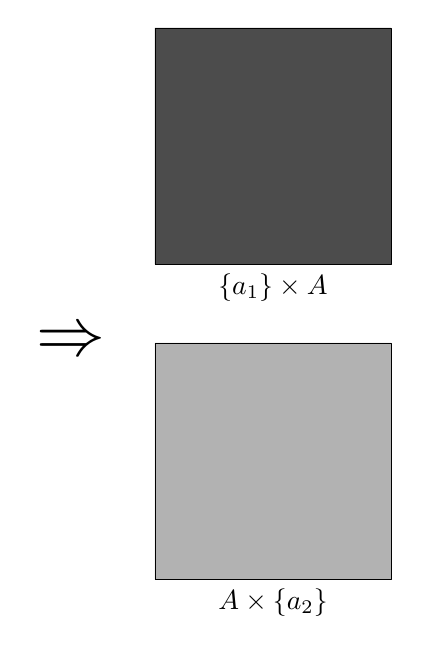
\begin{tikzpicture}
    \draw[very thin,black,line join=round,fill=black!30]
        (0,1) -- node [below,black] {$A \times \{a_2\}$} (3,1) -- node[right,black] {$\Gm$} (3,4) -- (0,4) -- (0,1);
    \draw[very thin,black,line join=round,fill=black!70]
        (0,5) -- node [below,black] {$\{a_1\} \times A$} (3,5) -- node[right,black] {$\Gm$} (3,8) -- (0,8) -- (0,5);
    \node[anchor=east] at (-0.5,4) {\Huge $\Rightarrow$};
\end{tikzpicture}
\end{center}
\caption{Extensions contained in a biextension.}
\end{figure}
There is a canonical piece of gluing data on this biextension, in the form of an isomorphism of pullback bundles
\begin{align*}
e_{p^j}\co (p^j \times 1)^* \L|_{A[p^j] \times A[p^j]} & \cong (1 \times p^j)^* \L|_{A[p^j] \times A[p^j]}, \\
(\ell, x, y) & \mapsto \left(\ell \cdot \prod_{k=1}^{p^j-1} \frac{s(x, [k]x, y)}{s(x, [k]y, y)} \right).
\end{align*}
This function $e_{p^j}$ is called the \textit{($p^j${\th}) Weil pairing}.
\end{definition}

\begin{remark}
In the case that $A$ is an elliptic curve, this agrees with the usual definition of its ``Weil pairing''. % In the case of an elliptic curve, this lines up with more traditional definitions --- for instance, using the isogeny $n: C \to C$.  In the case of a \emph{complex} elliptic curve $\C / (1, \tau)$, this degenerates further to the assignment \[\left( \frac{a}{n}, \frac{b}{n} \tau \right) \mapsto \exp\left(-2\pi i \frac{ab}{n}\right).\]
\end{remark}

\begin{lemma}\citeme{AS, I guess}
The Weil pairings assemble into a total Weil pairing on the $p$--divisible group associated to $A$.  Together, the total Weil pairing is alternating and biexponential. \qed
\end{lemma}

We can use the same formula in the setting of a cubical structure on a line bundle over a finite height formal group $\G$ to produce the desired map \[e_*\co C^3(\G; \Gm) \to \InternalHom{FormalGroups}(\G^{\wedge 2}, \Gm).\]  In fact, this is the right map:
\begin{lemma}[{\cite[Theorem 4.2, Corollary 4.4]{AndoStrickland}}]
The square commutes (up to sign):
\begin{center}
\begin{tikzcd}
\Spec E_0 BU[6, \infty) \arrow{r} \arrow{d}{\Pi_3} & \Spec E_0 K(\Z, 3) \arrow{d}{b_*} \\
C^3(\CP^\infty_E; \mathbb G_m) \arrow{r}{e} & \Weil(\CP^\infty_E).
\end{tikzcd}
\end{center}
\end{lemma}
\begin{proof}[Proof sketch]
This is reasonably difficult.  The main points are to show that the restriction \[d_{p^j}\co BC_{p^j}^{\times 2} \xrightarrow{\beta \circ \mu} \OS{H\Z}{3} \to BU[6, \infty)\] can be expressed by the Weil pairing formula: \[d_{p^j} = \bigoplus_{k=1}^{p^j-1} \left((\L_1 - 1)(\L_1^{\otimes k} - 1)(\L_2 - 1) - (\L_1 - 1)(\L_2^{\otimes k} - 1)(\L_2 - 1)\right).\]  After this is accomplished, what's left is to use naturality properties of the adjoint construction to compute the clockwise and counterclockwise composites.
\end{proof}

This fills out the diagram we are considering.  We now assemble just enough exactness results:

\begin{lemma}[{\cite[Lemma 7.2]{AndoStrickland}}]
The map $\delta\co C^2 \to C^3$ is injective for $\CP^\infty_E$ a finite height formal group.
\end{lemma}
\begin{proof}
Being finite height means that the multiplication-by-$p$ map of $\CP^\infty_E$ is fppf--surjective.  The kernel of $\delta$ consists of maps alternating, biexponential maps $(\CP^\infty_E)^{\times 2} \to \Gm$.  By restricting such a map $f$ to \[f \co \CP^\infty_E[p^j] \times \CP^\infty_E \to \Gm,\] we can calculate \[f(x, p^j y) = f(p^j x, y) = f(0, y) = 1.\]  But since $p^j$ is surjective on $\CP^\infty_E$, every point on the right-hand side can be so written, so at every left-hand stage the map is trivial.  Finally, $\CP^\infty_E = \colim_j \CP^\infty_E[p^j]$, so this filtration is exhaustive and we conclude that the kernel is trivial.
\end{proof}

\begin{lemma}[{\cite[Lemma 7.3]{AndoStrickland}}]
In fact, the following sequence is exact \[0 \to C^2(\CP^\infty_E; \Gm) \xrightarrow\delta C^3(\CP^\infty_E; \Gm) \to \Weil(\CP^\infty_E).\]
\end{lemma}
\begin{proof}
This is hard work.  Breen's idea is to show that picking a preimage under $\delta$ is the same as picking a trivialization of the underlying symmetric biextension of the cubical structure.  Then (following Mumford), one shows that the underlying symmetric biextension is trivial exactly if the Weil pairing is trivial.\todo{You could put in references here. AS gives them.}
\end{proof}

Finally, the top row falls quickly:

\begin{lemma}[{\cite[Lemma 7.5]{AndoStrickland}}]
\todo{Remark: This proof also shows that the $E$--theory of $\OS{kU}{8}$ fits into a sexseq.}
The top row of the main diagram is a short exact sequence of group schemes.
\end{lemma}
\begin{proof}
This is easiest proved by considering the sequence of homology Hopf algebras instead.  Since the integral homology of $BSU$ and the $E$--homology of $\OS{H\Z}{3}$ are both free and even, the Atiyah--Hirzebruch spectral sequence for $E_* BU[6, \infty)$ collapses.
\end{proof}

\begin{corollary}
The map \[\Pi_3\co \Spec E_0 BU[6, \infty) \to C^3(\CP^\infty_E; \Gm)\] is an isomorphism, and the map \[e_*\co C^3(\CP^\infty_E; \Gm) \to \InternalHom{FormalGroups}((\CP^\infty_E)^{\wedge 2}, \Gm)\] is a surjection.
\end{corollary}
\begin{proof}
This is a direct consequence of the $5$--lemma.
\end{proof}








% We begin with the fiber:

% \begin{lemma}[{\cite[Lemma 4.5]{AndoStrickland}}]\label{EasyCompatibilityWithdn}
% Write
% \begin{align*}
% d_n(\L_1, \L_2) & := \sum_{k=1}^{p^j-1} \left( (\L_1 - 1)(\L_1^k - 1)(\L_2 - 1) - (\L_1 - 1)(\L_2^k - 1)(\L_2 - 1)\right).
% \end{align*}
% There is a unique $\lambda \in \Z/n$ such that the following triangle commutes:
% \begin{center}
% \begin{tikzcd}
% (B\Z/p^j)^{\times 2} \arrow{d}{\lambda \beta \mu} \arrow{rd}{d_n(\L_1, \L_2)} \\
% K(\Z, 3) \arrow{r}{i} & BU[6, \infty).
% \end{tikzcd}
% \end{center}
% \end{lemma}
% \begin{proof}
% Forgetting down to $BU$ and working with just virtual bundles rather than lifts of virtual bundles to elements of $kU^6$, the definition of $d_n(\L_1, \L_2)$ gives
% \begin{align*}
% d_n(\L_1, \L_2) & = (\L_1 - 1)(\L_2^{p^j} - 1) - (\L_1^{p^k} - 1)(\L_2 - 1).
% \end{align*}
% Since we have restricted to $(B\Z/p^j)^{\times 2}$, $\L_1^{p^k} = 1$ and $\L_2^{p^k} = 1$, so this formula collapses and the composite map \[(B\Z/p^j)^{\times 2} \xrightarrow{d_n} BU[6, \infty) \xrightarrow{\pi_2} BSU \xrightarrow{\pi_2} BU\] is null.  We now study the lifting problem across the two maps:
% \begin{enumerate}
% \item[$\pi_1$:] Since the long composite is null, it follows that the shorter composite $\pi_2 \circ d_n$ factors through the fiber of $\pi_2$.  But, the fiber of $\pi_2$ is $S^1$, and there are no maps \[\{(B\Z/p^j)^{\times 2} \to S^1\} \cong H^1((B\Z/p^j)^{\times 2}; \Z) = 0.\]  It follows that $\pi_2 \circ d_n$ is itself null.
% \item[$\pi_2$:] Since $\pi_2 \circ d_n$ is null, $d_n$ must factor through the fiber of $\pi_2$, which is $K(\Z, 3)$.  With identical motives, one considers $H^3((B\Z/p^j)^{\times 2}; \Z)$, which is cyclic of order $n$ and generated by $\beta \circ \mu$. \qedhere
% \end{enumerate}
% \end{proof}

% \noindent This Lemma was missing a nontriviality statement, which turns out to be much harder:\todo{You could probably abbreviate the proof of this and include it.}

% \begin{theorem}[{\cite[Theorem 4.2, Section 5]{AndoStrickland}}]
% The value of $\lambda$ in \Cref{EasyCompatibilityWithdn} can be taken to be $\pm 1$. \qed
% \end{theorem}

% We now play one of our main cards: our willingness to work with cooperations means that we can pass from the hard task of checking facts about our formal schemes to the generally easier task of checking facts about their Cartier duals.  Because the formal schemes themselves are designed to have universal properties, their Cartier duals have points which are specified by these universal properties, and we win a considerable increase in tangibility.  In order to make full use of this, we record a mechanism of translation between these perspectives:


% These ideas power the following Lemma:

% \begin{proof}
% The target scheme $\Weil(\CP^\infty_E)$ is a subscheme of $\InternalHom{FormalGroups}((\CP^\infty_E)^{\times 2}, \Gm)$.  Since $\CP^\infty_E$ is finite height it satisfies $\CP^\infty_E = \colim_j \CP^\infty_E[p^j]$, which, coupled with the exponential adjunciton, reduces us to showing the agreement of the pair of composite maps \[\Spec E_0 BU[6, \infty) \times_{\S_E} \CP^\infty_E[p^j]^{\times 2} \to \Gm.\]  We will express these maps in terms of the adjoint map construction, starting with the clockwise composite.  The class $\beta \mu \in H\Z^3 BC_{p^j}^{\times 2}$ gives rise to an adjoint map \[\widehat{\beta \mu}\co \G_E[p^j]^{\times 2} \times (\OS{H\Z}{3})_E^\vee \to \Gm,\] which pulls back along $i\co \OS{H\Z}{3} \to \OS{kU}{6}$ to give \[(1 \times \Spec E_0 i) \circ \widehat{\beta \mu} = \widehat{i \beta \mu} = \widehat{d_n(\L_1, \L_2)}\] by the previous Theorem.

% We now try to calculate this adjoint, which will lead us to the counterclockwise composite.  First, the bundle $\bigotimes_{j=1}^3 (\L_j - 1) \in kU^6 (\CP^\infty)^{\times 3}$ gives rise to an adjoint map satisfying the following compatibility:
% \begin{center}
% \begin{tikzcd}
% (\CP^\infty_E)^{\times 3} \times \Spec E_0 BU[6, \infty) \arrow["\widehat{\bigotimes_{j=1}^3 (\L_j - 1)}"]{r} \arrow{d} & \Gm \\
% (\CP^\infty_E)^{\times 3} \times C^3(\CP^\infty_E; \Gm) \arrow{r} & (\CP^\infty_E)^{\times 3} \times \InternalHom{FormalSchemes}((\CP^\infty_E)^{\times 3}, \Gm) \arrow["\text{eval}"]{u}.
% \end{tikzcd}
% \end{center}
% The effect of postcomposing with the Weil pairing map can be viewed instead as precomposing the bottom-right corner with the






% \todo[inline]{This proof is unclear to the point of being broken.  How does the middle paragraph address the bottom-left arm of the square?}
% We will check compatibility on $\Weil_n(\CP^\infty_E)$ for arbitrary $n$, and so restrict from $i$ to $i \circ \lambda \beta \mu = d_n(\L_1, \L_2)$.
% % (Note: the sign can't bounce with $n$ because $\CP^\infty_E$ is $p$--divisible.)
% Since $\Weil_n(\CP^\infty_E)$ is a subscheme \[\Weil_n(\CP^\infty_E) \subseteq \InternalHom{FormalSchemes}(\CP^\infty_E[n]^{\times 2}, \Gm),\] we can push forward to checking equality here, i.e., of the two maps \[\Spec E_0 BU[6, \infty) \times_{\S_E} \CP^\infty_E[n]^{\times 2} \to \Gm.\]

% Writing $z = \prod_{i=1}^3 (1 - \L_i) \in kU^6 (\CP^\infty)^{\times 3}$, properties of the adjoint construction $\hat z$ show that it is given by the composite \[\hat z \co \Spec E_0 BU[6, \infty) \times_{\S_E} (\CP^\infty_E)^{\times 3} \to C^3(\CP^\infty_E; \Gm) \times_{\S_E} (\CP^\infty_E)^{\times 3} \xrightarrow{\operatorname{eval}} \Gm.\]  By specializing to $z = (1 - \L_1)(1 - \L_1^k)(1 - \L_2) \in kU^6 (\CP^\infty)^{\times 2}$, we see that $\hat z$ acts by\todo{Do I mean to be writing $k$--series here? I think I do.} \[\hat z \co (f, (g_1, g_2)) \mapsto f(g_1, [k](g_1), g_2),\] and continuing along these lines we see \[\widehat{d_n(\L_1, \L_2)} \co (f, (g_1, g_2)) \mapsto \prod_{k=1}^{n-1} \frac{f(g_1, [k](g_1), g_2)}{f(g_1, [k](g_2), g_2)} = e_n(f)(g_1, g_2).\]

% That described the bottom-left arm of the square.  The other way around the square is easier: take $w = \beta \circ \mu \in H^3(B\Z/p^j)^{\times 2}$ with adjoint $\hat w \co \CP^\infty_E[p^j]^{\times 2} \times K(\Z, 3)^E \to \Gm$.  Naturality shows $\hat w \circ \gamma^E = \widehat{\gamma_* w}$, and the theorem shows $\gamma_* w = \pm d_n(\L_1, \L_2)$, hence $\widehat{\gamma_* w} = (\pm d_n(\L_1, \L_2))\hat{}$, which is adjoint to $(e_n \Pi_3)^\pm$.
% \end{proof}

% \todo{There's a nice construction of the $\Pi_k$ maps in the AHS preprint where the ``$C_k$'' constructions are performed directly on the spectra, then applying $(-)_E$ carries those constructions to relevant constructions on group schemes, and finally Cartier duality gives the maps $\Pi_k$ of the sort described above.  This is superior to saying ``adjoint'', in my opinion, though it could be remarked that these are equivalent.}
% \todo{Consider including Lemma 6.2 and so on, the $BSU \to BU$ equivalents of the later statements you need.}

% % \begin{lemma}[{\cite[Lemma 6.2]{AndoStrickland}}]
% % The adjoint of the map $E_0 \CP^\infty \to E_0 BU$ induces a map $\Pi_1: BU^E \to C^1(\CP^\infty_E; \mathbb G_m)$ which is an isomorphism.  In fact, the Cartier duality isomorphism $(\CP^\infty)^E \cong \InternalHom{FormalGroups}(\CP^\infty_E, \mathbb G_m)$ fits into a commuting square
% % \begin{center}
% % \begin{tikzcd}
% % (\CP^\infty)^E \arrow{r} \arrow{d} & \InternalHom{FormalGroups}(\CP^\infty_E, \Gm) \arrow{d}{\begin{array}{c} \text{natural} \\ \text{inclusion} \end{array}} \\
% % BU^E \arrow{r}{\Pi_1} & C^1(\CP^\infty_E; \Gm).
% % \end{tikzcd}
% % \end{center}
% % \end{lemma}
% % \begin{proof}
% % \todo{Include this.}
% % \end{proof}

% % \begin{theorem}\label{BUBSUandC1C2Commute}
% % The following square commutes:
% % \begin{center}
% % \begin{tikzcd}
% % BU^E \arrow{d}{\Pi_1} \arrow{r} & BSU^E \arrow{d}{\Pi_2} \\
% % C^1(\CP^\infty_E; \Gm) \arrow{r}{\delta} & C^2(\CP^\infty_E; \Gm).
% % \end{tikzcd}
% % \end{center}
% % \end{theorem}
% % \begin{proof}
% % \citeme{Lemma 6.4 of AS}
% % This is a matter of expanding definitions and using \[(\L_1 - 1)(\L_2 - 1) = \mu^*(\L - 1) - \pi_1^*(\L - 1) - \pi_2(\L - 1).\]
% % \end{proof}

% % \begin{theorem}
% % The following is a map of short exact sequences:
% % \begin{center}
% % \begin{tikzcd}
% % 0 \arrow{r} & (\CP^\infty)^E \arrow{d} \arrow{r} & BU^E \arrow{r} \arrow{d} & BSU^E \arrow{r} \arrow{d} & 0 \\
% % 0 \arrow{r} & \InternalHom{FormalGroups}(\CP^\infty_E; \Gm) \arrow{r} & C^1(\CP^\infty; \Gm) \arrow{r} & C^2(\CP^\infty; \Gm) \arrow{r} & 0.
% % \end{tikzcd}
% % \end{center}
% % \end{theorem}
% % \begin{proof}
% % \citeme{Prop 6.5 of AS. They reference a superior alternate argument in the AHS preprint though\ldots}
% % \end{proof}








\section{Unstable additive cooperations for $kU$}

Write $H = H\F_p$.  Today we will study the effect of the map $\hat \Pi_3$ in ordinary homology.  Many parts of the proof we explored for $E$--theory break.  Topologically, the Serre spectral sequence for $H^* BU[6, \infty)$ is not even-concentrated and so is not forced to collapse.  Algebraically, because $\G_a$ is not $p$--divisible the behavior of the model exact sequence is also suspect.  Because the situation has fewer insulating good properties, we are forced to actually consider it carefully.  The upside, however, is that the standard group law on $\G_a$ is simple enough that we can compute the problem to death.

We begin with the topological half of our tasks.  The Serre spectral sequence \[E_2^{*, *} = H\F_p^* BSU \otimes H\F_p^* \OS{H\Z}{3}) \Rightarrow H\F_p^* BU[6, \infty)\] is quite accessible, and we will recount the case of $p = 2$.  In this case, the spectral sequence has $E_2$--page \[E_2^{*, *} = H\F_2^* BSU \otimes H\F_2^* \OS{H\Z}{3} \cong \F_2[c_2, c_3, \ldots] \otimes \F_2\left[\Sq^I \iota_3 \middle| \begin{array}{c} I_j \ge 2I_{j+1}, \\ 2 I_1 - I_+ \end{array}\right].\]  Because the target is $6$--connective, we must have the transgressive differential $d_4 \iota_3 = c_2$, which via the Kudo transgression theorem spurs the much larger family of differentials \[d_{4+I_+} \Sq^I \iota_3 = \Sq^I c_2.\]  This necessitates understanding the action of the Steenrod operations on the cohomology of $BSU$, which is due to Wu\citeme{Wu formulas, maybe May's concise book}:\todo{Can these formulas be read off from the divisorial calculation?  Maybe not, since it's easy to read off the Milnor primitives but harder to see the Steenrod squares.} \[\Sq^{2^j} \cdots \Sq^4 \Sq^2 c_2 = c_{1 + 2^j}.\]  Accounting for the squares of classes left behind, this culminates in the following calculation:\todo{This spectral sequence can be drawn in using Hood's package.}

\begin{theorem}\label{HF2BU6Calculation}
There is an isomorphism \[H\F_2^* BU[6, \infty) \cong \frac{H\F_2^* BU}{(c_j \mid j \ne 2^k + 1, j \ge 3)} \otimes F_2[\iota_3^2, (\Sq^2 \iota_3)^2, \ldots]. \qed\]
\end{theorem}

\begin{theorem}\citeme{Stong, Singer}
More generally, there is an isomorphism \[H\F_2^* \OS{kU}{2k} \cong \frac{H\F_2^* BU}{(c_j \mid \sigma_2(j - 1) < k - 1)} \otimes \operatorname{Op}[\Sq^3 \iota_{2k-1}],\] where $\sigma_2$ is the dyadic digital sum and ``$\operatorname{Op}$'' denotes the subalgebra of $H\F_2^* \OS{H\Z}{2k-1}$ generated by the indicated class.
\end{theorem}
\begin{proof}[Remarks on proof]
Stong specialized to $p = 2$ and carefully applied the Serre spectral sequence to the fibrations \[\OS{kU}{2(k+1)} \to \OS{kU}{2k} \to \OS{H\Z}{2k}.\]  Singer worked at an arbitrary prime and used the Eilenberg--Moore spectral sequence for the fibrations \[\OS{H\Z}{2k-1} \to \OS{kU}{2(k+1)} \to \OS{kU}{2k}.\]  Both used considerable knowledge of the interaction of these spectral sequences with the Steenrod algebra.
\end{proof}

\begin{remark}
These methods and results generalize directly to odd primes.  The necessary modifications come from understanding the unstable mod--$p$ Steenrod algebra, using the analogues of Wu's formulas due to Shay\citeme{Wu formulas, Shay's extension in \textit{mod--$p$ Wu formulas for the Steenrod algebra and the Dyer--Lashof algebra}}, and employing Singer's Eilenberg--Moore calculation.  Again, $H\F_p^* BU[6, \infty)$ is presented as a quotient by $H\F_p^* BU$ by certain Chern classes satisfying a $p$--adic sum condition, tensored up with the subalgebra of $H\F_p^* \OS{H\Z}{3}$ generated by a certain element.
\end{remark}

\begin{remark}
We can already see from \Cref{HF2BU6Calculation} that our map of short exact sequences in \Cref{ChromaticKUCoopnsSection} does not have a full analogue in the setting of additive homology.  By considering the edge homomorphism in the Serre spectral sequence, we see that \[\Spec HP_0 BSU \to \Spec HP_0 BU[6, \infty)\] is not a monomorphism.
\end{remark}





Now, we turn to the algebra.  The main idea, as already used in \Cref{CalculationOfLTTangentSpace}, is to first perform a tangent space calculation of \[T_0 C^k(\G_a; \Gm) \cong C^k(\G_a; \G_a),\] then study the behavior of the different tangent directions to determine the full object $C^k(\G_a; \Gm)$.  As a warm-up, we will first consider the case $k = 2$:
\begin{corollary}[{cf.\ \Cref{CohomologyOfGa}}]
The unique symmetric $2$--cocycle of homogeneous degree $n$ has the form \[c_n(x, y) = \begin{cases} (x + y)^n - x^n - y^n & \text{if $n \ne p^j$}, \\ \frac{1}{p} \left( (x + y)^n - x^n - y^n \right) & \text{if $n = p^j$}. \end{cases} \qed\]
\end{corollary}

Our goal, then, is to select such a $2$--cocycle $f$ and study the minimal conditions needed on a symbol $a$ to produce a multiplicative $2$--cocycle of the form $1 + af + \cdots$.  Since $c_n = \frac{1}{d_n} \delta(x^n)$ is itself produced by an additive formula, life would be easiest if we had access to an exponential, so that we could build \[\text{``$ \delta \exp(a_n x^n)^{1/d_n} = \exp(\delta a_n x^n / d_n) = \exp(a_n c_n). $''}\]  However, the existence of an exponential series is equivalent to requiring that $a_n$ have all fractions, which turns out not to be minimal.  In fact, \emph{no} conditions on $a_n$ are required \emph{at all}, if we tweak the definition of an exponential series:

\begin{definition}\todo{Where does this come from? I've never learned a universal property for it. That bothers me. It must have something to do with $p$--typification.}
The \textit{Artin--Hasse exponential} is the power series \[E_p(t) = \exp\left( \sum_{j=0}^\infty \frac{t^{p^j}}{p^j} \right) \in \Z_{(p)}\ps{t}.\]
\end{definition}

This series has excellent properties, mimicking those of $\exp(t)$ as closely as possible while keeping coefficients in $\Z_{(p)}$ rather than in $\Q$.  Writing $\delta\co C^1 \to C^2$ and \[d_n = \begin{cases} 1 & \text{if $n = p^j$}, \\ 0 & \text{otherwise}, \end{cases}\] we set \[g_n(x, y) := \delta E_p(a_n x^n)^{1/p^{d_n}} = \exp\left( \sum_{j=0}^\infty \frac{a_n^{p^j} \delta x^{np^j}}{p^{j + d_n}} \right) = \exp\left( \sum_{j=0}^\infty \frac{a_n^{p^j} c_{np^j}(x, y)}{p^j} \right).\]  This gives a point in $C^2(\G_a; \Gm)(\Z_{(p)}[a_n])$, and exhaustion of the tangent space proves the following Lemma:

\begin{lemma}[{\cite[Proposition 3.9]{AHSTheoremOfTheCube}}]
The map \[\Spec \Z_{(p)}[a_n \mid n \ge 2] \xrightarrow{\prod_{n \ge 2} g_2} C^2(\G_a; \Gm) \times \Spec \Z_{(p)}\] is an isomorphism. \qed
\end{lemma}

The case $k = 3$ is similar, with one important new wrinkle.  Over an $\F_2$--algebra there is an equality $c_n^2 = c_{2n}$.  However, this relation does not generalize to trivariate $2$--cocycles:
\begin{align*}
\frac{1}{2} \delta (c_6) & = x^2 y^2 z^2 + x^4 y z + x y^4 z + x y z^4, &
\left(\frac{1}{2} \delta c_3\right)^2 & = x^2 y^2 z^2.
\end{align*}
This pattern is generic and exhaustive for $\F_p$--algebras:
\begin{lemma}[{\cite[Proposition 3.20, Proposition A.12]{AHSTheoremOfTheCube}}]
The $p$--primary residue of the scheme of trivariate symmetric $2$--cocycles is presented by \[\Spec \F_p[a_d \mid d \ge 3] \times \Spec \F_p[b_d \mid d = p^j(1 + p^k)] \xrightarrow{\cong} C^3(\G_a; \G_a) \times \Spec \F_p. \qed\]
\end{lemma}

\noindent Similar juggling of the Artin--Hasse exponential yields the following multiplicative classification:
\begin{theorem}[{\cite[Proposition 3.28]{AHSTheoremOfTheCube}}]
There is an isomorphism \[\Spec \Z_{(p)}[a_d \mid d \ge 3, d \ne 1 + p^t] \times \Spec \Gamma[b_{1 + p^t}] \xrightarrow{} C^3(\G_a; \Gm) \times \Spec \Z_{(p)}.\]
\end{theorem}
\begin{proof}[Proof sketch]
The main claim is that the Artin--Hasse exponential trick used in the case $k = 2$ works here as well, provided $d \ne 1 + p^t$ so that taking an appropriate $p${\th} root works out.  They then show that the remaining exceptional cases extend to multiplicative cocycles only when the $p${\th} power of the leading coefficient vanishes.  Finally, a rational calculation shows how to bind these truncated generators together into a divided power algebra.
\end{proof}

In our pursuit of the map of exact sequences of \Cref{ChromaticKUCoopnsSection}, we are missing one piece: a link from topology to the scheme of Weil pairings, $\Weil(\G_a)$.  The object ``$\Spec HP_0 \OS{H\Z}{3}$'' is insuitable because it doesn't exist --- the homology algebra $HP_0 \OS{H\Z}{3}$ is not even--concentrated.  However, analyzing the edge homomorphism from our governing Serre spectral sequence shows that the map \[HP^0 BU[6, \infty) \to HP^0 \OS{H\Z}{3}\] factors through the subalgebra $A$ generated by the \emph{squares} of the polynomial generators.  Accordingly, we aim to place $\Spec A^*$ in the top-right corner of our map of 

\begin{lemma}[{\cite[Lemma 3.36, Proposition 4.13, Lemma 4.11]{AHSTheoremOfTheCube}}]
The scheme $\Spec A^*$ models $\Weil(\G_a)$ by an isomorphism $\lambda$ commuting with $e \circ \hat \Pi_3$.
\end{lemma}
\begin{proof}[Proof sketch]
The $\F_p$--scheme $\Weil(\G_a)$ is simple to describe:
\begin{center}
\begin{tikzcd}[row sep=1em]
(a_{mn})_{m, n} \arrow[|->]{r} & \prod_{m < n} \operatorname{texp}\left(a_{mn}(x^{p^m} y^{p^n} - x^{p^n} y^{p^m})\right) \\
\Spec \F_p[a_{mn} \mid m < n] / (a_{mn}^p) \arrow{r}{\cong} & \Weil(\G_a),
\end{tikzcd}
\end{center}
where $\operatorname{texp}(t) = \sum_{j=0}^{p-1} t^j / j!$ is the truncated exponential series.  It is easy to check that this ring of functions agrees with $A^*$, and it requires hard work (although not much creativity) to check the remainder of the statement: that $e \circ \hat \Pi_3$ factors through $\Spec A^*$ and that the factorization is an isomorphism.
\end{proof}

We have now finally assembled our map of right-exact sequences:\todo{It's maybe not obvious to a reader why this sequence is exact in the middle, although you have secretly proven this in the mess above.}
\begin{center}
\begin{tikzcd}
\Spec HP_0 BSU \arrow{r} \arrow["\hat \Pi_2", "\cong"']{d} & \Spec HP_0 BU[6, \infty) \arrow{r} \arrow["\hat \Pi_3"]{d} & \Spec A^* \arrow{r} \arrow["\lambda", "\cong"']{d} & 0 \\
C^2(\G_a; \Gm) \arrow{r}{\delta} & C^3(\G_a; \Gm) \arrow{r}{e} & \Weil(\G_a) \arrow{r} & 0.
\end{tikzcd}
\end{center}
Our calculations now pay off:
\begin{corollary}
The map $\hat \Pi_3$ is an isomorphism: \[\hat \Pi_3\co \Spec HP_0 BU[6, \infty) \xrightarrow{\cong} C^3(\G_a; \Gm).\]
\end{corollary}
\begin{proof}[Proof sketch]
The main point is that we don't actually have to compute much about the middle map.  Because the squares commute and the sequences are exact as indicated, we at least learn that $\hat \Pi_3$ is an epimorphism after base-change to $\Spec \Q$ and $\Spec \F_p$ for each prime $p$.  But, since both source and target are affine schemes of graded finite type with equal Poincar\'e series in each case, our epimorphism is an isomorphism.
\end{proof}

\begin{corollary}[{\cite[Theorem 2.31]{AHSTheoremOfTheCube}}]\label{Pi3ForCplxOrientableE}
The map $\hat \Pi_3$ is an isomorphism for any complex-orientable $E$.\todo{Jay asked in class for a summary of exactly what exactness statements are true for a general $E$ (especially relative to the extreme case of $E$--theory, where everything is exact and pleasant).}
\end{corollary}
\begin{proof}[Proof sketch]
This follows much along the lines of \Cref{HopfRingForEBP}.  We check that the statement holds for $E = MUP$ using a tangent space argument, and then an Atiyah--Hirzebruch argument gives the statement for any complex-oriented $E$.
\end{proof}

\begin{remark}
Our analysis in \Cref{LEFTCooperations} gives us full access to the Hopf ring structure of the \emph{nonconnective} cooperations $H\F_p{}_* \OS{KU}{2*}$.  Using a variety of techniques, Morton and Strickland calculated the Hopf ring structure of $H\F_2{}_* \OS{K}{2*}$ where $K$ ranges among the nonconnective objects $KO$, $KU$, $KSp$, and the less common ``$KT$'', which is self--conjugated $K$--theory~\cite{Morton,MortonStrickland,StricklandBottPeriodicity}.\todo{This could be expanded some, as not all these references are relevant to what's written.}
\end{remark}










\section{Covariance, $\Theta$--structures on Thom sheaves}

Today we will (despite appearances) mostly leave the algebraic geometry alone, instead attending to two lingering topological concerns.  First, over the past few lectures we have been concerned with the homology schemes $\Spec E_0 \OS{kU}{2*}$.  We were originally motivated by a sequence of cohomological isomorphisms
\begin{align*}
(BU \times \Z)_E & \cong \Sym^0_{\Div \CP^\infty_E} \Div_0 \CP^\infty_E =: C_0 \CP^\infty_E, \\
BU_E & \cong \Sym^1_{\Div \CP^\infty_E} \Div_0 \CP^\infty_E =: C_1 \CP^\infty_E, \\
BSU_E & \cong \Sym^2_{\Div \CP^\infty_E} \Div_0 \CP^\infty_E =: C_2 \CP^\infty_E,
\end{align*}
along with identifications
\begin{align*}
BU \times \Z & \simeq \OS{kU}{2 \cdot 0}, &
BU & \simeq \OS{kU}{2 \cdot 1}, &
BSU & \simeq \OS{kU}{2 \cdot 2}.
\end{align*}
Our analysis of Cartier duality in \Cref{TopologicalCartierDuality} gave us isomorphisms like \[\Spec E_0 BSU \cong \InternalHom{GroupSchemes}(BSU_E, \Gm) \cong \InternalHom{FormalGroups}(C_2 \CP^\infty_E, \G_m).\] Following the universal property of this particular symmetric square, we were led to consider the scheme of symmetric bivariate functions on $\CP^\infty_E$ satisfying a $2$--cocycle condition.  Our next move was to show that $\Spec E_0 BU[6, \infty)$ was modeled by a similar scheme of \emph{trivariate} functions --- but we proved this directly, while avoiding the ``predual'' cohomological statement \[BU[6, \infty)_E \cong C_3 \CP^\infty_E := \Sym^3_{\Div \CP^\infty_E} \Div_0 \CP^\infty_E.\]  This is because the homological statement is the low-hanging fruit: it is easy to demonstrate that the scheme of such functions exists as a closed subscheme of all functions.  It is considerably harder to show that a symmetric cube exists at all.

\begin{lemma}\label{CkGaGmAreFVars}\citeme{4.41 in the AHS preprint}
$DC^k(\G_a; \Gm)$ are all formal varieties for $k \le 3$.
\end{lemma}
\begin{proof}
We know that $\sheaf O C^k(\G_a; \Gm)$ are all free $\Z$--modules of graded finite rank in the range $k \le 3$, so we may write \[\sheaf O(D C^k(\G_a; \Gm)) \cong (\sheaf O C^k(\G_a; \Gm))^*.\]  We will show that this later Hopf algebra $\sheaf O(C^k(\G_a; \Gm))^*$ is a power series ring, specializing for the moment to the case $k = 2$.  It will suffice to show that it is a power series ring modulo $p$ for every prime $p$.  Such graded connected finite-type Hopf algebras over $\F_p$ were classified by Borel (and exposited by Milnor--Moore~\cite[Theorem 7.11]{MilnorMoore}) as either polynomial or truncated polynomial.  These two cases are distinguished by the Frobenius operation: the Frobenius on a polynomial ring is injective, whereas the Frobenius on a truncated polynomial ring is not.  It is therefore equivalent to show that the \emph{Verschiebung} on the original ring $\sheaf O(C^2(\G_a; \Gm)) \otimes \F_p$ is \emph{surjective}.  Recalling that $c_n^p = c_{np}$ at the level of bivariate $2$--cocycles, we compute \[p^* a_n = a_{np}^p,\] and since $F a_{np} = a_{np}^p$ and $FV = p^*$, we learn \[V(a_{np}) = a_n.\]

Essentially the same proof handles the cases $k = 1$ and $k = 0$.  The case $k = 3$ requires a small modification, to cope with the two classes of trivariate $2$--cocycles.  On the polynomial tensor factor of $\sheaf O(C^3(\G_a; \Gm))$ we can reuse the same Verschiebung argument to see that its dual Hopf algebra is polynomial.  The dual of the divided power tensor factor is immediately a primitively generated polynomial algebra, without any further argument.
\end{proof}

\begin{theorem}
The scheme $C_3 \CP^\infty_E$ exists, and it is modeled by $BU[6, \infty)_E$.
\end{theorem}
\begin{proof}[Proof sketch]
\todo{This regurgitated proof is pretty broken.}
\citeme{Prop 3.3 in AHS preprint}
Let $\G$ be an arbitrary formal group.  Note first that if $C^3(\G; \Gm)$ is coalgebraic, then $C_3 \G$ exists and is its Cartier dual: the diagram presenting $\sheaf O(C^3(\G; \Gm))$ as a reflexive coequalizer of free Hopf algebras is also the diagram meant to present $C_3 \G$ as a coalgebraic formal scheme.  So, if the coequalizing Hopf algebra has a good basis, it will follow from \Cref{CoalgebraicColimitsExist} that the resulting diagram is a colimit diagram in formal schemes, with $C_3 \G$ sitting at the cone point.  It will additionally follow from there that the isomorphism from \Cref{Pi3ForCplxOrientableE} \[\Spec E_0 BU[6, \infty) \xrightarrow{\cong} C^3(\CP^\infty_E; \Gm)\] will re-dualize to an isomorphism \[BU[6, \infty)_E \xleftarrow{\cong} C_3 \CP^\infty_E.\]

\citeme{Prop 3.4 in the AHS preprint}
\todo{Here we are again, making grading arguments. We've been bad about this earlier in the paper too.}
So, we reduce to checking that $\sheaf O(C^3(\G; \Gm))$ admits a good basis.  By a base change argument, it suffices to take $\G$ to be the universal formal group over the Lazard ring.  Noting that $\sheaf O(C^3(\G; \Gm))$ must be of graded finite type, we will work to show that it is free on a basis we have good control over.

Specializing from $\G$ over $\moduli{fgl}$ to $\G_a$ over $\Spec \Z$, we know from \Cref{CkGaGmAreFVars} that $\sheaf O(C^3(\G_a; \Gm))$ is a free abelian group, and we know from \Cref{LazardsTheorem} that $\sheaf O(\moduli{fgl})$ is as well.  By picking a $\Z$--basis $\Z\{\beta_j\}_j$ of $\sheaf O C^3(\G_a; \Gm)$, we can choose a map of $\sheaf O(\moduli{fgl})$--modules lifting it
\begin{center}
\begin{tikzcd}
\sheaf O(\moduli{fgl})\{\tilde \beta_j\}_j \arrow["\alpha"]{r} \arrow{d} & \sheaf O C^3(\G; \Gm) \arrow{d} \\
\Z\{\beta_j\}_j \arrow["\cong"]{r} & \sheaf O C^3(\G_a; \Gm).
\end{tikzcd}
\end{center}
By induction on degree, one sees that $\alpha$ is surjective, and since the source is a free abelian group we need only check that the source and target have the same Poincar\'e series to conclude that $\alpha$ is an isomorphism.

We proceed to test this rationally: over $\Spec \Q$ we can use the logarithm to construct an isomorphism \[\Spec \Q \times (\moduli{fgl} \times C^k(\G; \Gm)) \to \Spec \Q \times (\moduli{fgl} \times C^k(\G_a; \Gm)),\] hence the Poincar\'e series agree, so $\alpha \otimes \Q$ and $\alpha$ are both isomorphisms.  Having established freenss, our other goal was to show that $M$ has a sequence of good subcoalgebras.  These come by considering the subcoalgebras, indexed on an integer $d$, spanned by the basis vectors of degree at most $d$.
\end{proof}

Our second task today is to address the gap between $\OS{kU}{2k}$ and its Thom spectrum $T(\OS{kU}{2k})$.  After all, our motivation for all of this algebraic geometry is to give a description to the set \[(\Spec E_0 MU[6, \infty))(E_0),\] but what we have done so far is describe the scheme $\Spec E_0 BU[6, \infty)$.  Since these two spectra are related by a Thom construction, we should be able to deduce the description that we want by thinking about Thom sheaves.  We now straighten this out.  The place to start is with a construction:

\begin{lemma}
For $\xi\co G \to BGL_1 \S$ a group map, the Thom spectrum $T\xi$ is a $(\Susp^\infty_+ G)$--cotorsor.
\end{lemma}
\begin{proof}[Proof sketch]
The Thom isomorphism $T\xi \sm T\xi \simeq T\xi \sm \Susp^\infty_+ G$ composes with the unit map $\S \to T\xi$ to give the \textit{Thom diagonal} \[T\xi \to T\xi \sm \Susp^\infty_+ G. \qedhere\]
\end{proof}

\begin{corollary}
In addition to our interpretation of $\ThomSheaf{\xi}$ as a $\Gm$--torsor over $G_E$, $\ThomSheaf{\xi}^{-1}$ is furthermore a $(G_E \times \Gm)$--torsor over $S_E$. \qed
\end{corollary}

We expand this idea out in our situation.  A morphism $MU[6, \infty) \to E$ produces a trivialization of $\ThomSheaf{\bigotimes_{j=1}^3 (\L_j - 1)}$ over $(\CP^\infty_E)^{\times 3}$, and the associated trivializing section is symmetric and rigid\citeme{Lemma 2.49 of AHS}.  This prompts us to make the following definition:

\begin{definition}
We write $C^k(\G; \sheaf L)$ for the functor of trivializing sections of $\Theta^k \sheaf L$ over $\G^{\times k}$ which are symmetric and rigid.  This construction has some nice properties:
\begin{itemize}
\item Note that taking the trivial sheaf $\sheaf L = \sheaf O_{\G}$ recovers the scheme $C^k(\G; \Gm)$ of $\Gm$--valued such functions from before.
\item By consequence, if $\sheaf L$ is \emph{trivializable} then this functor is an affine scheme.
\item Affine or not, there is a pairing map \[C^k(\G; \sheaf L) \times C^k(\G; \sheaf H) \to C^k(\G; \sheaf L \otimes \sheaf H).\]  In particular, this recovers the group structure on $C^k(\G; \Gm)$ and it makes $C^k(\G; \sheaf L)$ into a $C^k(\G; \Gm)$--torsor.
\end{itemize}
\end{definition}

\noindent Thus, we have constructed a map \[\phi\co \Spec E_0 MU[6, \infty) \to C^3(\CP^\infty_E; \sheaf I(0)).\] The following Lemma is a matter of fully expanding definitions:

\begin{lemma}[{\cite[Theorem 2.50]{AHSTheoremOfTheCube}}]
The map \[\Spec E_0 MU[6, \infty) \to C^3(\CP^\infty_E; \sheaf I(0))\] is an isomorphism.
\end{lemma}
\begin{proof}[Proof sketch]
\todo{You shouldn't call this anything more than a ``proof sketch'' unless you expand out the reasoning for why this square commutes.}
This map is equivariant, in the sense that the following square commutes:
\begin{center}
\begin{tikzcd}
\Spec E_0 MU[6, \infty) \times \Spec E_0 BU[6, \infty) \arrow{r} \arrow{d}{\phi \times \text{\ref{Pi3ForCplxOrientableE}}} & \Spec E_0 MU[6, \infty) \arrow{d}{\phi} \\
C^3(\CP^\infty_E; \sheaf I(0)) \times C^3(\CP^\infty_E; \Gm) \arrow{r} & C^3(\CP^\infty_E; \sheaf I(0)).
\end{tikzcd}
\end{center}
Any equivariant map of torsors is automatically an isomorphism.
\end{proof}

\noindent This, finally, gives us access to the analogue of \Cref{BUZTriumvirate}, \Cref{BUTriumvirate}, and \Cref{BSUTriumvirate}:

\begin{corollary}\label{BU6Triumvirate}
Take $E$ to be \emph{complex--orientable}.  The functor $C^3(\CP^\infty_E; \sheaf I(0))$ defined by
\begin{align*}
\CatOf{AffineSchemes}_{/\Spec E_0} & \to \CatOf{Sets}, \\
(\Spec T \xrightarrow{u} \Spec E_0) & \mapsto \left\{ \begin{array}{c} \text{symmetric, rigid trivializations} \\ \text{of $u^* \Theta^3 \ThomSheaf{\L}$ over $u^* (\CP^\infty_E)^{\times 3}$} \end{array} \right\}
\end{align*}
is isomorphic to the affine scheme $\Spec E_0 MU[6, \infty)$.  Moreover, the $E_0$--points of this scheme biject with ring spectrum maps $MU[6, \infty) \to E$. \qed
\end{corollary}

\todo{This is a leftover todo from the following section.  We accomplish all of this here, but I haven't looked at the references tacked on at the end of this to see if they say anything I've missed.  --- --- --- --- --- I want to sketch the reduction for even-periodic elliptic cohomology theories to the case of $MUP$, then from there to $HkP$ for the prime fields $K$, then from there to questions about additive cocycles.  We certainly don't need to recall any of these calculations, but I think it's a nice example of the philosophy that the additive formal group is such a knotted point of $\moduli{fg}$ that it suffices to check something there to learn it for the rest of the stack.  This survives in the published form of AHS, but it's stated pretty clearly as Prop 3.4 in the unpublished verison.  See also 5.12 of the unpublished version.}

% \begin{remark}\todo[color=red]{Actually work this out.}
% It should be possible to give an example of a complex-oriented theory which receives an $MSU$ orientation which \emph{does not} factor the complex orientation but \emph{does} (\emph{must}, really) factor the unit?  Even if one can find an example of this, I think it will be somewhat artificial: the sequence of group schemes \[0 \to BSU_E \to BU_E \to BU(1)_E \to 0\] is short exact, \emph{and} it has a splitting on the level of formal schemes.  The splitting is what gives you the isomorphism on points $BSU_E(T) \times BU(1)_E(T) \cong BU_E(T)$.  On the other hand, because the splitting \emph{isn't} a map of formal groups, it doesn't survive to the Cartier dual short exact sequence \[0 \from BSU^E \from BU^E \from BU(1)^E \from 0,\] so this will come down to exhibiting a test ring $T = E_*$ for which $BU^E(T) \to BSU^E(T)$, despite being induced by an fppf-surjective map of sheaves, is not surjective on sections over $T$.  Of course, this comes down concretely to solving for a preimage under the map \[1 - g(x) \mapsto \frac{1 - g(x +_{\G} y)}{(1 - g(x))(1 - g(y))},\] which is more plodding but might offer insight into what sort of ring (and thus orientation) you're looking for.
% \end{remark}












\section{Modular forms from $MU[6, \infty)$--manifolds}

Our goal today is to actually leverage the arithmetic geometry in \Cref{Theta3IsTrivial}, rather than just using the body of results about $\theta$--functions as inspiration.  In order to do this, we need to place ourselves in a situation where algebraic topology is directly linked to abelian varieties.

\begin{definition}\label{DefnEllipticSpectrum}
An \textit{elliptic spectrum} consists of a even--periodic ring spectrum $E$, a (generalized) elliptic curve $C$ over $\Spec E_0$, and a fixed isomorphism \[\phi\co C^\wedge_0 \xrightarrow{\cong} \CP^\infty_E.\]  A map among such spectra consists of a map of ring spectra $f\co E \to E'$ together with a specified isomorphism of elliptic curves $\psi\co f^* C \to C'$.
\end{definition}

\begin{remark}
We have chosen to consider \emph{isomorphisms} of elliptic curve rather than general homomorphisms because this is what algebraic topology suggests that we do.  After all, the mixed cooperations of complex-oriented ring spectra are modeled by the isomorphisms of the associated formal groups.  In the next Case Study, we will develop a theory (with an attendant notion of a ``context'') which incorporates isogenies of elliptic curves in addition to isomorphisms.
\end{remark}

Coupling \Cref{DefnEllipticSpectrum} to \Cref{BU6Triumvirate} and \Cref{Theta3IsTrivial}, we learn the following result:
\begin{corollary}\label{EllipticSpectraAreOriented}
An elliptic spectrum $(E, C, \phi)$ receives a canonical map of ring spectra \[MU[6, \infty) \to E.\]  This map is natural in choice of elliptic spectrum: if $(E, C, \phi) \to (E', C', \phi')$ is a map of elliptic spectra, then the triangle
\begin{center}
\begin{tikzcd}
& MU[6, \infty) \arrow{ld} \arrow{rd} \\
E \arrow{rr} & & E'
\end{tikzcd}
\end{center}
commutes. \qed
\end{corollary}

\begin{example}
Our basic example of an elliptic curve was $E_\Lambda = \C / \Lambda$, with $\Lambda$ a complex lattice.  The projection $\C \to \C / \Lambda$ has a local inverse which defines an isomorphism of formal groups \[\phi\co (E_\Lambda)^\wedge_0 \xrightarrow{\cong} \G_a \otimes \C.\]  Accordingly, we define an elliptic spectrum $HE_\Lambda P$ whose underlying ring spectrum is $H\C$ and whose associated elliptic curve and isomorphism are $E_\Lambda$ and $\phi$.  This spectrum receives a natural map \[MU[6, \infty) \to HE_\Lambda P,\] which to a bordism class $M \in MU[6, \infty)_{2n}$ assigns an element $\Phi_\Lambda(M) \cdot u_\Lambda^n \in HE_\Lambda P_{2n}$ for some $\Phi_\Lambda(M) \in \C$.
\end{example}

\begin{example}
The naturality of the $MU[6, \infty)$--orientation moves us to consider more than one elliptic spectrum at a time.  If $\Lambda'$ is another lattice with $\Lambda' = \lambda \cdot \Lambda$, then the multiplication map $\lambda\co \C \to \C$ descends to an isomorphism $E_\Lambda \to E_{\Lambda'}$ and hence a map of elliptic spectra $HE_{\Lambda'}P \to HE_\Lambda P$ acting by $u_{\Lambda'} \mapsto \lambda u_\Lambda$.  The commuting triangle in \Cref{EllipticSpectraAreOriented} then begets the \emph{modularity relation} \[\Phi(M; \lambda \cdot \Lambda) = \lambda^{-n} \Phi(M; \Lambda).\]
\end{example}

\begin{example}\label{OrdinaryHomologyInUpperHalfPlaneEx}
This equation leads us to consider all curves $E_\Lambda$ simultaneously --- or, equivalently, to consider modular forms.  The lattice $\Lambda$ can be put into a standard form, by picking a basis and scaling it so that one vector lies at $1$ and the other vector lies in the upper half-plane.  This gives a cover \[\h \to \moduli{ell} \times \Spec \C\] which is well-behaved away from the special points $i$ and $e^{2 \pi i / 6}$.  A \textit{complex modular form of weight $k$} is an analytic function $\h \to \C$ which satisfies a certain decay condition and which is quasi-periodic for the action of $SL_2(\Z)$, i.e.,\footnote{That is, for the action of change of basis vectors.} \[f\left(M; \frac{a \tau + b}{c \tau + d} \right) = (c \tau + d)^n f(M; \tau).\]

Using these ideas, we construct a cohomology theory $H \sheaf O_{\h} P$, where $\sheaf O_{\h}$ is the ring of complex-analytic functions on the upper half-plane.  The $\h$--parametrized family of elliptic curves \[\h \times \C / (1, \tau) \to \h,\] together with the logarithm, present $H \sheaf O_{\h} P$ as an elliptic spectrum $H\h P$.  The canonical map $\Phi\co MU[6, \infty) \to H\h P$ specializes at a point to give the functions $\Phi(-; \Lambda)$ considered above, and hence $\Phi(M)$ is itself a complex modular form of weight $k$.
\end{example}

In fact, this is a ghost of Ochanine and Witten's modular genus from \Cref{OchanineWittenTheorem}, as a bordism class in $MU[6, \infty)_{2n}$ is, in particular, a bordism class in $M\String_{2n}$.  However, they know more about this function than we can presently see: they claim that it has an integral $q$--expansion.  In terms of the modular form, its $q$--expansion is given by building the Taylor expansion ``at $\infty$'' (using that unspoken decay condition).  In order to use our topological methods, it would be nice to have an elliptic spectrum embodying these $q$--expansions in the same way that $H\h P$ embodied holomorphic functions, together with a comparison map that trades a modular form for its $q$--expansion.  The main ideas leading to such a spectrum come from considering the behavior of $E_\Lambda$ as $\tau$ tends to $i \cdot \infty$.

\begin{definition}
Note that as $\tau \to i \cdot \infty$, the parameter $q = \exp(2 \pi i \tau)$ tends to $0$.  In the multiplicative model of \Cref{SectionEllipticCurvesAndThetaFunctions}, we considered $D'$ the punctured complex disk with associated family of elliptic curves \[C'_{\mathrm{an}} = \C^\times \times D' / (u, q) \sim (qu, q).\]  The fiber of $C'$ over a particular point $q \in D'$ is the curve $\C^\times / q^{\Z}$. %  , and $\theta$ determines a holomorphic function on the total space $\C^\times \times D'$.
The Weierstrass equations give an embedding of $C'_{\mathrm{an}}$ into $D' \times \CP^2$ described by \[wy^2 + wxy = x^3 - 5 \alpha_3 w^2 x + -\frac{5 \alpha_3 + 7 \alpha_5}{12}w^3\] for certain functions\todo{Do these have weights?} $\alpha_3$ and $\alpha_5$ of $q$.  At $q = 0$, these curve collapses to the twisted cubic \[wy^2 + wxy = x^3,\] and over the whole open unit disc $D$ we call this extended family $C_{\mathrm{an}}$.

Now let $A \subseteq \Z\ps{q}$ by the subring of power series which converge absolutely on the open unit disk.  It turns out that the coefficients of the Weierstrass cubic (i.e., $5\alpha_3$ and $\frac{1}{12}(5\alpha_3+7\alpha_5)$) lie in $A$, so it determines a generalized elliptic curve $C$ over $\Spec A$, and $C_{\mathrm{an}}$ is the curve given by base-change from $A$ to the ring of holomorphic functions on $D$.\citeme{Find a reference for this. You may be able to look in Morava's Section 5}  The \textit{Tate curve} $C_{\Tate}$ is defined to be the family over the intermediate object $D_{\Tate} = \Spec \Z\ps{q}$ base-changed from $A$.
\end{definition}

The singular fiber at $q = 0$ prompts us to enlarge our notion of elliptic curve slightly.

\begin{definition}[{\cite[Definitions B.1-2]{AHSTheoremOfTheCube}}]\citeme{Is this right? Check the published AHS to make sure}
\todo{Erick didn't like the name ``generalized elliptic curve'', which already means something else in arithmetic (disallowing cuspidal singularities and also allowing other funny behavior). He didn't have a second suggestion, though.}
A \textit{Weierstrass curve} is \emph{any} curve of the form\todo{You use $w$s above but $z$s here.} \[C(a_1, a_2, a_3, a_4, a_6) := \left\{ ([x : y : z], s) \in \mathbb P^2 \times S \middle| \begin{array}{c} y^2 z + a_1(s) xyz + a_3(s) yz^2 = \\ x^3 + a_2(s) x^2 z + a_4(s) x z^2 + a_6(s) z^3 \end{array} \right\}.\]  A \textit{generalized elliptic curve} over $S$ is a scheme $C$ equipped with maps \[S \xrightarrow{0} C \xrightarrow{\pi} S\] such that $C$ is Zariski--locally isomorphic to a system of Weierstrass curves (in a way preserving $0$ and $\pi$).\footnote{An elliptic curve in the usual sense turns out to be a generalized elliptic curve which is smooth, i.e., the discriminant of the Weierstrass equations is a unit.}
\end{definition}

\begin{remark}\label{TwistedCubicGivesGm}\citeme{Some kind of reference would be appreciated}
The singularities of a degenerate Weierstrass equation always occur outside of a formal neighborhood of the marked identity point, which in fact still carries the structure of a formal group.  The formal group associated to the twisted cubic is the multiplicative group\todo{The smooth locus of the twisted cubic is actually also the \emph{informal} multiplicative group.  The $\theta$--function we're going to describe below also has the property that it specializes at $q = 0$ to the usual coordinate $(1 - u)$ on $\Gm$, which is nice.  This degeneracy to honest--$\Gm$ is probably also related to the use of the Todd orientation further down.}, and the isomorphism making the identification extends a family of such isomorphisms $\phi$ over the nonsingular part of the Tate curve.
\end{remark}

\begin{definition}[{\cite[Section 5]{MoravaFormsOfKthy}, \cite[Section 2.7]{AHSTheoremOfTheCube}}]
The elliptic spectrum $K_{\Tate}$, called \textit{Tate $K$--theory}, has as its underlying spectrum $KU\ps{q}$.  The associated elliptic curve is $C_{\Tate}$, and the isomorphism $\CP^\infty_{KU\ps{q}} \cong (C_{\Tate})^\wedge_0$ is $\phi$ from \Cref{TwistedCubicGivesGm}.
\end{definition}

\noindent The trade for the breadth of this definition is that theorems pulled from the study of abelian varities have to be shown to extend uniquely to those generalized elliptic curves which are not smooth curves.

\begin{theorem}[{\cite[Propositions 2.57 and B.25]{AHSTheoremOfTheCube}}]\label{GeneralizedTheta3IsTrivial}
For a generalized elliptic curve $C$, there is a canonical\todo{You should compare this with the unicity statement in the previous iteration of this theorem, plus how it's \emph{not} unique at these singular points.} trivialization $s$ of $\Theta^3 \sheaf I(0)$ which is compatible with change of base and with isomorphisms.  If $C$ is a smooth elliptic curve, then $s$ agrees with that of \Cref{Theta3IsTrivial}. \qed
\end{theorem}

\begin{corollary}\label{D3thetaTrivializes}
The trivializing section $s$ associated to $C_{\Tate}$ is given by $\delta^{\circ 3} \theta$, where\todo{This is a little funny, because this is \emph{not} one of the usual $\theta$--functions from \Cref{SectionEllipticCurvesAndThetaFunctions}.  I think we should state its quasiperiodicity relation again, since it doesn't agree with the old one.} \[\theta_q(u) = (1 - u)\prod_{n > 0}(1 - q^n u)(1 - q^n u^{-1}).\]
\end{corollary}
\begin{proof}
Even though $\theta$ is not a function on $C_{\Tate}$ because of quasiperiodicity, it does trivialize both $\pi^* \sheaf I(0)$ for $\pi\co \C^\times \times D \to C_{\Tate}$ and $\sheaf I(0)$ for $(C_{\Tate})^\wedge_0$.  Moreover, the quasiperiodicities in the factors in the formula defining $\delta^3 \theta|_{(C_{\Tate})^\wedge_0}$ cancel each other out, and the function does descend to give a trivialization of $\Theta^3 \sheaf I(0)$.  By the unicity clause in \Cref{GeneralizedTheta3IsTrivial}, it must give a formula expressing $s$.\todo{This use of unicity is a little opaque to me.  I guess we're using that $\delta^3 \theta$ is ``obviously'' the natural trivializing section for nonsingular values of $q$?  Or maybe we just mean that the Tate curve covers much of $\moduli{ell} \times \Spec \C$.}
\end{proof}

\begin{definition}
The induced map \[\sigma_{\Tate}\co MU[6, \infty) \to K_{\Tate}\] is called the \textit{complex $\sigma$--orientation}.
\end{definition}

\begin{corollary}\label{WittensTheoremForBU6}
Let $M \in \pi_{2n} MU[6, \infty)$ be a bordism class.  The $q$--expansion of Witten's modular form $\Phi(M)$ has integral coefficients.
\end{corollary}
\begin{proof}
The span of elliptic spectra equipped with $MU[6, \infty)$--orientations
\begin{center}
\begin{tikzcd}
& MU[6, \infty) \arrow["\Phi"]{rd} \arrow{d} \arrow["\sigma_{\Tate}"']{ld} \\
K_{\Tate} \arrow{r} & K_{\Tate} \otimes \C & H\h P \arrow{l}
\end{tikzcd}
\end{center}
models $q$--expansion.  The arrow $K_{\Tate} \to K_{\Tate} \otimes \C$ is injective on homotopy, which shows that the $q$--expansion of $\Phi(M)$ lands in the subring of integral power series.
\end{proof}

In fact, \Cref{D3thetaTrivializes} gives us access to a formula for $\sigma_{\Tate} = \delta^3 \theta$, where $\theta$ here is interpreted as a coordinate on $(C_{\Tate})^\wedge_0$.  This means that $\sigma_{\Tate}$ belongs to the commutative triangle
\begin{center}
\begin{tikzcd}
MU[6, \infty) \arrow["\delta"']{d} \arrow["\sigma_{\Tate}"]{drrr} \\
MSU \arrow["\delta"']{r} & MU \arrow["\delta"']{r} & MUP \arrow["\theta"']{r} & K\ps{q}.
\end{tikzcd}
\end{center}
To begin, the usual map $MUP \to KU$ selects the coordinate $f(u) = 1 - u$ on the formal completion of $\Gm = \Spec \Z[u^\pm]$.  The induced map \[MU \xrightarrow{\delta} MUP \to KU\] sends $f$ to the rigid section $\delta f$ of \[\Theta^1 \sheaf I(0) = \sheaf I(0)_0 \otimes \sheaf I(0)^{-1} \cong \omega \otimes \sheaf I(0),\] and in terms of the right-hand side, \[\delta f = \frac{f'(0)}{f(u)} Du = \frac{1}{1 - u} \left( - \frac{du}{u} \right),\] where $Du$ is the invariant differential.  We can augment this to a calculation of $\delta \theta$ by considering the composite \todo{This first map is one of the units.  Which is it?} \[\delta \theta\co MU \xrightarrow{\eta_R} MU \sm MU \simeq MU \sm BU_+ \xrightarrow{\delta(1 - u) \sm \theta'} K_{\Tate}\] where $\theta'$ is the element of $BU^{K_{\Tate}} \cong C^1(\widehat C_{\Tate}; \Gm)$ given by the formula\todo{I'm confused.  Where did this class come from? Is it the derivative of $\theta$?  The $\delta$--derivative of $\theta$?  Something else? Actually, it sort of looks like $(1 - u) \cdot \theta(1) / \theta(u)$...?} \[\theta' = \prod_{n \ge 1} \frac{(1 - q^n)^2}{(1 - q^n u)(1 - q^n u^{-1})}.\]  This means that its effect on a line bundle is determined by \[\theta'(1 - \L) = \prod_{n \ge 1} \frac{(1 - q^n)^2}{(1 - q^n \L)(1 - q^n \L^{-1})},\] and its effect on vector bundles in general is determined by the splitting principle and an exponential law.  In fact, one can work this exponential law out to mean \[\theta'(\dim V \cdot 1 - V) = \bigotimes_{n \ge 1} \bigoplus_{j \ge 0} \Sym^j(\dim V \cdot 1 - V \otimes_{\R} \C) q^{jn} =: \bigotimes_{n \ge 1} \Sym_{q^n}(- \bar V_{\C}).\]

Knowing that $(\eta_R)_*\co MU_* \to \pi_*(MU \sm \Susp^\infty_+ BU)$ sends a manifold $M$ with stable normal bundle $\nu$ to the pair $(M, \nu)$, we compute the composite on homotopy to be
\begin{align*}
\sigma_{\Tate}(M \in \pi_{2n} MU[6, \infty)) & = (\delta(1-u) \sm \theta')(M, \nu) \\
& =: \Td\left(M; \bigotimes_{n \ge 1} \Sym_{q^n}(\bar \tau_{\C}) \right).
\end{align*}
This is exactly Witten's formula for his genus, as applied to complex manifolds with first two Chern classes trivialized.

\todo[inline]{This is missing something.  We have written $\Td(M) (-du/u)^n$ for $MU_{2n} \to KU_{2n}$, the effect in homotopy of the usual coordinate on $KU$.  You can also think of this as $p_! 1$ for $1 \in K^{2n} M$ and $p\co M \to *$.  More generally, then, $\Td(M; V) := p_! V$.  But, also, we did describe pushforwards earlier... maybe we can make use of this?}













\section{$\Spin$ and $\String$ orientations}

\todo[inline]{A different approach to this is to work through the $p \ne 2$ case, since you can totally, correctly work it out and see the $\Sigma$--structure relation get imposed. That's kind of attractive.  Too bad you had this through after the class was complete.}

In the previous Lecture, we proved that elliptic spectra receive canonical $MU[6, \infty)$--orientations, that complex elliptic spectra collectively give rise to a genus valued in modular forms, and that the $q$--expansions of these modular forms are integral.  However, the original \Cref{OchanineWittenTheorem} of Ochanine and Witten claimed to describe a genus on $\Spin$-- and $\String$--manifolds, which we have only managed to approximate with our study of $MU[6, \infty)$--orientations.  Our last goal for this Case Study is to show that the chromatic formal schemes associated to spaces like $B\String$ are somewhat accessible, and so chromatically-amenable elliptic spectra receive canonical $M\String$--orientations.

Fix a formal group $\Gamma$ of finite height $d$, and write $K = K_\Gamma$ for the associated Morava $K$--theory.  We will start with the more modest goal of understanding the bottom few layers of the Postnikov tower for $\OS{kO}{0} \simeq BO \times \Z$, which have the names
\begin{align*}
BO[2, \infty) & := BSO, &
BO[4, \infty) & := B\Spin, &
BO[8, \infty) & := B\String.
\end{align*}

\begin{remark}
Unlike $kU$, there is \emph{not} an equivalence \[\OS{kO}{n} \not\simeq (BO \times \Z)[n, \infty),\] unless $n$ happens to take the form $n = 8k$ for a nonnegative integer $k$.  The reasoning for this stray equivalence is similar to that for $kU$: the homotopy ring of $kO$ has a polynomial factor of degree $8$, and the other elements lie in a band of dimensions smaller than $8$.  Otherwise, other things happen --- for instance,
\begin{align*}
\OS{kO}{1} & \simeq O/U, &
\OS{kO}{6} & \simeq \Spin / SU.
\end{align*}
\end{remark}

\begin{remark}[{\cite[Section 5.2]{KLW}}]
We may as well take the ground field of our Morava $K$--theory to have characteristic $p = 2$, since at odd characteristics there is little distinction between $kO$ and $kU$, owing to the fiber sequence \[\Susp kO \xrightarrow{\cdot \eta = 0} kO \to kU.\]  However, this reveals a disadvantage of Morava $K$--theory that will finally cause us real consternation: Morava $K$--theories at the prime $2$ are not commutative ring spectra.  Accordingly, $(K_\Gamma)_* G$ for a commutative $H$--group $G$ may fail to give a commutative algebra.  Luckily, \Cref{MoravaKIsNotCommutative} tells us that if $(K_\Gamma)_* G$ happens to be even-concentrated, then the obstructions to commutativity identically vanish.  So, we can be somewhat indelicate about this noncommutativity issue, provided that we continually check that the algebras we are forming are even-concentrated.
\end{remark}

In order to get off the ground, we will need the following Lemma about the behavior of the Atiyah--Hirzebruch spectral sequence for a Morava $K$--theory:
\begin{lemma}[{\cite[Lemma 2.1]{Yagita}}]\label{MoravaKThyAHSS}
\todo{Does this Lemma admit a coordinate-free statement? They probably aren't all identically controlled by $Q_d$, but rather by $Q_d$ plus decomposables.}
Let $k_\Gamma$ be the connective cover of the Morava $K$--theory $K_\Gamma$.  In the Atiyah--Hirzebruch spectral sequence \[E_2^{*, *} = Hk^* X \otimes_k k_\Gamma^* \Rightarrow k_\Gamma^* X,\] the differentials are given by \[d_r(x) = \begin{cases} 0 & \text{if $r \le 2(p^d - 1)$}, \\ \lambda Q_d x \otimes v_d & \text{if $r = 2(p^d - 1) + 1$} \end{cases}\] where $\lambda \ne 0$ and $Q_d$ is the $d${\th} Milnor primitive. \qed
\end{lemma}

\begin{corollary}[{\cite[Section 2.5]{RWY}, \cite[Equation 3.1]{KLW}}]\label{FormalSchemeForBO}
There is a bi-Cartesian square of coalgebraic formal schemes
\begin{center}
\begin{tikzcd}
& \Div_0 \barG[2] \arrow{rr} \arrow{ld} & & \Div_0 \G[2] \arrow{ld} \\
\Div_0 \barG \arrow{rr} & & BO_K.
\end{tikzcd}
\end{center}
\end{corollary}
\begin{proof}
We apply \Cref{MoravaKThyAHSS} to the analysis of the spectral sequence of Hopf algebras \[H\F_2{}_* BO \otimes (K_\Gamma)_* \Rightarrow (K_\Gamma)_* BO.\]  \citeme{I don't know where these Milnor primitives are calculated. I guess we could have done them using formal geometry} We have $H\F_2{}_* BO \cong \F_2[b_1, b_2, \ldots]$ and \[Q_d b_{2^{d+1} + 2j} = b_{2j + 1},\] from which it follows that all the odd generators are killed, all their squares survive, and only the even generators of low degree are permanent cycles.  This results in a decomposition \[(K_\Gamma)_* BO \cong (K_\Gamma)_*[b_2, b_4, b_{2^{d+1}-2}] \underset{(K_\Gamma)[b_{2j}^2 \mid j < 2^d]}{\otimes} (K_\Gamma)_*[b_{2j}^2],\] and so we are tasked with assigning names to the coalgebraic formal schemes appearing in this formula.

The left-hand factor is the free Hopf algebra on the coalgebra determined by the $2$--torsion in the formal group $\Gamma$.  The right-hand factor is the free Hopf algebra on the formal curve $\barG := \HP^\infty_K$, using the isogeny
\begin{align*}
\HP^\infty_K & \to \CP^\infty_K \\
y & \mapsto x \cdot [-1](x)
\end{align*}
induced by desymplectification.  Because $\H^\times$ is not commutative, $\barG$ is not a formal group, but we pull back the multiplication-by-$2$ isogeny from $\G$ to $\barG$ and define the subscheme $\barG[2]$ of points mapping to zero.
\end{proof}

Suppose that the Postnikov sections \[X(n, \infty) \to X[n, \infty) \to X[n, n]\] induce short exact sequences of formal groups.  A presentation of $X_K$ as a bi-Cartesian square then acquires value via the following algebraic Lemma:

\begin{lemma}\label{CubeOfFibers}
Consider the cube of formal group schemes constructed by taking pointwise fibers of the composite to $G$:
\begin{center}
\begin{tikzcd}
& A' \arrow{rr} \arrow{ld} \arrow{dd} & & B' \arrow{ld} \arrow{dd} \\
C' \arrow[crossing over]{rr} \arrow{dd} & & D' \\
& A \arrow{rr} \arrow{ld} & & B \arrow{ld} \\
C \arrow{rr} & & D \arrow{rr} \arrow[leftarrow, crossing over]{uu} & & G.
\end{tikzcd}
\end{center}
If the bottom face is bi-Cartesian, then so is the top. \qed
\end{lemma}

\begin{corollary}\label{BSpinAnalysis}
There is a bi-Cartesian square
\begin{center}
\begin{tikzcd}
& \Div_0 \barG[2] \arrow{rr} \arrow{ld} & & \SDiv_0 \G[2] \arrow{ld} \\
\Div_0 \barG \arrow{rr} & & BSO_K.
\end{tikzcd}
\end{center}
\end{corollary}
\begin{proof}[Proof sketch]
The fibration $BSO \to BO \to BO(1)$ gives a short exact sequence of Hopf algebras, so using \Cref{FormalSchemeForBO} we are in the situation of \Cref{CubeOfFibers}.  To compute the pointwise kernels, begin by considering the commuting square of Postnikov sections
\begin{center}
\begin{tikzcd}
BO_K \arrow{r} \arrow{d} & BU_K \arrow{d} \\
\G[2] \arrow{r} & \G.
\end{tikzcd}
\end{center}
Both horizontal maps are injections.  Since $\Div \barG \to BU_K \cong \Div_0 \G \to \G$ is null, the composite $\Div_0 \barG \to \G[2]$ is null.  Similarly, the composite $\Div \G[2] \to \G[2]$ acts by summation, and its kernel is $\SDiv_0 \G[2]$.
\end{proof}

From here, the computation gets harder.  

\begin{corollary}[{\cite[Section 5.3]{KLW}}]
There is a bi-Cartesian square
\begin{center}
\begin{tikzcd}
& \Div_0 \barG[2] \arrow{rr} \arrow{ld} & & \ker \omega \arrow{ld} \\
\Div_0 \barG \arrow{rr} & & B\Spin_K,
\end{tikzcd}
\end{center}
where $\omega\co C_2 \G \to \G[2]^{\wedge 2}$ is the map $([a] - [0])([b] - [0]) \mapsto a \wedge b$.
\end{corollary}
\begin{proof}
This goes similarly to \Cref{BSpinAnalysis}, once you know that the Postnikov section induces a short exact sequence of formal groups\citeme{Cite the relevant part of KLW}.  The composite $\Div \barG \to \G[2]^{\wedge 2}$ is shown to be zero using an identical technique\todo{Really? This is what I have written down in my notes, but I can't expand it out.}.  To identify the behavior on the other factor, we need the following diagram of exact sequences of Hopf algebras from Kitchloo, Laures, and Wilson~\cite[Theorem 6.4]{KLW}:
\begin{center}
\begin{tikzcd}
& & & K_* \arrow{d} \\
& K_* \arrow{d} & & K_* K(\Z, 3) \arrow{d} \arrow[leftarrow, in=0, out=180, densely dotted]{llddd} \\
K_* \arrow{r} & K_* B\Spin \arrow{r} \arrow{d} & K_* BSU \arrow{r}{\tau} \arrow[equal]{d} & K_* BU[6, \infty) \arrow{d}{\delta} \\
K_* \arrow{r} & K_* BSO \arrow{r}{i} \arrow{d} & K_* BSU \arrow{r}{1 - \xi} & K_* BSU \arrow{d} \\
& K_* K(C_2, 2) \arrow{d} & & K_* \\
& K_*,
\end{tikzcd}
\end{center}
where $\tau\co C_2 \G \to C_3 \G$ is specified at the level of formal schemes by \[\tau\co ([a] - [0])([b] - [0]) \mapsto ([a] - [0])([b] - [0])([-a-b] - [0]).\]  Since $(1 - \xi) \circ i = 0$, we have that $\delta \circ \tau \circ i = 0$ and hence that $\tau \circ i$ lifts to $K_* K(\Z, 3)$.  Identifying $\SDiv_0 \G[2]$ with $C_2 \G[2]$, we check that the composites \[C_2 \G[2] \xrightarrow{\omega} \G[2]^{\wedge 2} \xrightarrow{\eps} C_3 \G\] and \[C_2 \G[2] \to C_2 \G \xrightarrow{\tau} C_3 \G\] agree.  For a point $[a, b] \in C_2 \G$, this is the claim
\begin{align*}
0 & = \eps(a \wedge b) - \tau[a, b] \\
& = [a, a, b] - [b, a, b] - [-a - b, a, b] \\
& = [a, a, b] - [b + a, a, b] + [b, a + a, b] - [b, a, b],
\end{align*}
and this is forced null in $C_3 \G$, as it looks like a $2$--cocycle shuffle.

\todo[inline]{I'm a little fuzzy on the coherence of this with the Bockstein: this computes the lift of $\tau \circ f$ into $K(\Z, 3)_K$, and it does happen to factor through the subscheme $K(\Z/2, 2)_K$ determined by the Bockstein. However, I don't immediately see why this agrees with the bottom Postnikov section of $BSO$: that's a map off of $BSO$ and this is a rotated map into $BU[6, \infty)$, so it's not an immediate consequence of naturality.  It has to do with rotating the Wood cofiber sequence just right, and in particular where the horizontal sequences come from: they're stitched-together from two consecutive Wood cofiber sequences.}
\end{proof}



\textbf{Ideally, we would use this presentation of $B\Spin_K$ to say something about $M\Spin$--orientations.  I just realized I don't know how, though!}



\begin{remark}
This computation becomes almost unfeasible for $B\String$, but we will sketch two approaches.  One is that the sequence \[\OS{HC_2}{2} \to \OS{HC_{2^\infty}}{2} \to B\String \to B\Spin \to \OS{HC_{2^\infty}}{4} \xrightarrow{2} \OS{HC_{2^\infty}}{4}\] induces an exact sequence of group schemes.  The other avenue of access is the pair of fiber sequences
\begin{align*}
\OS{H\Z}{3} & \to \widetilde{B\Spin} \to B\Spin, &
B\String & \to \widetilde{B\Spin} \to \OS{HC_2}{3},
\end{align*}
formed by considering the pullback of the corner \[B\Spin \to \OS{H\Z}{4} \from \OS{HC_2}{3}.\]  Both of these fibrations induce short exact sequences of Hopf algebras.
\end{remark}

However, since we are specifically interested in $M\String$--orientations, there is an alternative approach that avoids describing the formal scheme $B\String_K$.  Again appealing to results of Kitchloo, Laures, and Wilson, we find that the sequence \[K_* \Spin/SU \to K_* BU[6, \infty) \to K_* B\String\] is exact and right-exact\citeme{KLW}.  The kernel of the map $K_* \Spin/SU \to K_* BU[6, \infty)$ is a Hopf algebra they call ``$CK_3$'' \citeme{Theorem 2.3.5.vi of KLW}, where \[CK_j = \bigoplus_{k=j}^\infty K_* K(\Z/2, k).\]  More than that, KLW even say where the polynomial and nonpolynomial parts of $K_* \Spin/SU$ land inside of $K_* BU[6, \infty)$.  I think\todo{But I have not checked!} that this means that $K_* BU[6, \infty)$ is a flat $K_* \Spin/SU$--module at heights $d \le 2$.

Applying the Thom spectrum functor to the fiber square gives the pushout diagram
\begin{center}
\begin{tikzcd}
\Susp^\infty_+ \Spin/SU \arrow{r} \arrow{d} & MU[6, \infty) \arrow{d} \\
\S \arrow{r} & M\String,
\end{tikzcd}
\end{center}
or, equivalently, an equivalence \[M\String \simeq MU[6, \infty) \sm_{\Susp^\infty_+ \Spin/SU} \S.\]  This in turn gives a $\Tor$ spectral sequence of signature \[\Tor^{K_* \Spin/SU}_{*, *}(K_* MU[6, \infty), K_*) \Rightarrow K_* M\String.\]  So, under the flatness hypothesis above, there are no higher $\Tor$ terms so the spectral sequence collapses to give \[K_* M\String \cong K_* MU[6, \infty) \mmod K_* \Spin/SU.\]  So, what remains to be shown is that $K_* \Spin/SU$ picks out the correct extra relation for $\Sigma$--structures.  Then, we need a density argument to show that this handles all of the at-a-point cases of elliptic cohomology.













\begin{remark}
However, the spectra $HE_\Lambda P$ do not qualify as ``chromatically amenable'' from the perspective of this last argument, and so we lose access to our genus valued in modular forms.  Additionally, $K_{\Tate}$ does not qualify, essentially because it is integral rather than $p$--adic.  The methods described here give rise to putative $p$--adic $q$--expansions of modular forms, but we have not been able to check that they satisfy the modularity condition, nor that they assemble into a single, integral object.  Amazingly, such theorems are achievable, and they are the impetus for the study of topological modular forms and algebraic geometry done with $E_\infty$--rings.\todo{Expand this last sentence.  Point to the Appendix, or cite the $\TMF$ book, or idk.}
\end{remark}









\todo{The Atiyah--Bott--Shapiro orientation and the fibration $BSU \to B\Spin$.  This is possibly somewhere around Theorem 2.3.5.iv in KLW, the last fibration in 2.3.2 at $k=-2$, and sections 5.3 and 5.13}

\todo{Cite Kitchloo--Laures's ``Real structures and Morava $K$--theories''}

\todo{What follows is the analysis for $M\String$.  Is the one for $M\Spin$ analogous and do-able?  Does it involve $CK_2$ and maybe a clever choice of $MSU$--orientation?}

\todo{If you managed to get all this to work, you could try to understand the $M\Spin$--orientation of $K_{\Tate}$, as in page 628 of the published AHS.}









\subsection*{Some other things that might belong in this chapter}

The cubical structure on a singular (generalized) elliptic curve is not unique, but (published) AHS has an argument showing that the unicity of the choice on the nonsingular ``bulk'' extends to a unique choice on the ``boundary'' of the compactified moduli too.


There's also the work of Ando--French--Ganter on factorized / iterated $\Theta$ structures and how they give rise to the ``two--variable Jacobi genus''.












